%% ============================================================
%% Applying OAuth 2.1 Token Exchange with Nested Actor Claims
%% to MCP Agentic Workflows
%% Approximate word count (excl. abstract, references, captions): ~8500
%% v8 — Review fixes: figure* placement, table citations, theorem labels,
%%       removed mcp_wiki/vaswani2017/google_a2a, removed non-IEEE sections,
%%       fixed Auth0/PKCE claim, comms dual-audience note, language quality
%%
%% Compile: pdflatex (run twice for cross-references)
%% Packages: IEEEtran (journal), tikz, pgfplots,
%%           booktabs, multirow, colortbl, tabularx,
%%           amsmath (multline)
%% ============================================================
\documentclass[journal]{IEEEtran}
\IEEEoverridecommandlockouts

\usepackage[T1]{fontenc}
\usepackage{cite}
\usepackage{amsmath,amssymb,amsfonts}
\usepackage{graphicx}
\usepackage{textcomp}
\usepackage{xcolor}
\usepackage{booktabs}
\usepackage{url}
\usepackage{hyperref}
\usepackage{listings}
\usepackage{upquote}    %% straight quotes in listings (not curly)
\usepackage{multirow}
\usepackage{array}
\usepackage{tikz}
\usepackage{pgfplots}
\usepackage{colortbl}
\usepackage{tabularx}
\usepackage{balance}
\usepackage{placeins}   %% \FloatBarrier — prevents floats crossing section boundaries
%% amsthm provides \begin{proof} and \theoremstyle; compatible with IEEEtran
\usepackage{amsthm}
\newtheorem{theorem}{Design Property}          %% "Design Property 1", etc.
\newtheorem{proposition}{Proposition}           %% separate counter
\theoremstyle{definition}
\newtheorem{definition}{Definition}             %% upright body text

\usetikzlibrary{
  arrows.meta, shapes, positioning, fit,
  backgrounds, calc, decorations.pathreplacing,
  decorations.text
}
\pgfplotsset{compat=1.18}
\usepgfplotslibrary{groupplots}

\hypersetup{colorlinks=true,linkcolor=blue,citecolor=blue,urlcolor=blue}

%% ── colour palette ──────────────────────────────────────────
\definecolor{C_BASE}{HTML}{E07B54}  % warm orange – insecure / baseline
\definecolor{C_SEC} {HTML}{4C9BE8}  % cool blue   – NAC / secure
\definecolor{C_PAR} {HTML}{5DBB7A}  % green       – blocked / parallel
\definecolor{C_WARN}{HTML}{E74C3C}  % red         – attack / warning
\definecolor{C_HEAD}{HTML}{2C3E50}  % dark navy   – headers
\definecolor{SD_BG} {HTML}{EBF4FF}  % light blue  – sequence actor bg

%% ── code listing style ──────────────────────────────────────
\lstset{
  basicstyle=\fontsize{7}{8.4}\selectfont\ttfamily,
  breaklines=true,
  breakatwhitespace=true,
  frame=single,
  captionpos=b,
  xleftmargin=0.8em,
  numbers=left,
  numberstyle=\tiny\color{gray},
  numbersep=4pt,
  columns=flexible,
  keepspaces=true,
  showstringspaces=false,
}

%% ── global TikZ styles ──────────────────────────────────────
\tikzset{
  %% -- sequence diagram actors --
  SD/actor/.style={
    draw=C_HEAD!60, rounded corners=3pt,
    fill=SD_BG, minimum width=2.3cm, minimum height=0.58cm,
    align=center, font=\scriptsize\bfseries
  },
  %% -- sequence diagram lifeline --
  SD/life/.style={draw, dashed, gray!55, thin},
  %% -- sequence diagram forward arrow --
  SD/fwd/.style={-{Stealth[length=3.5pt]}, thick, color=C_HEAD!80},
  %% -- sequence diagram response arrow --
  SD/bck/.style={-{Stealth[length=3.5pt]}, thick, dashed, color=gray!65},
  %% -- sequence diagram message label --
  SD/lbl/.style={font=\tiny, fill=white, inner sep=1.5pt, align=center},
  %% -- sequence diagram "par" combined fragment --
  SD/par/.style={draw=gray, dashed, thick, rounded corners=2pt},
  %% -- generic box (architecture diagrams) --
  arch/hub/.style={
    draw, rounded corners=4pt, fill=C_SEC!18,
    minimum width=1.9cm, minimum height=0.6cm,
    align=center, font=\scriptsize\bfseries
  },
  arch/worker/.style={
    draw, rounded corners=4pt, fill=C_PAR!22,
    minimum width=1.6cm, minimum height=0.55cm,
    align=center, font=\scriptsize
  },
  arch/oauth/.style={
    draw, rounded corners=4pt, fill=C_BASE!18,
    minimum width=1.9cm, minimum height=0.6cm,
    align=center, font=\scriptsize\bfseries
  },
  arch/user/.style={
    draw, rounded corners=4pt, fill=gray!14,
    minimum width=1.4cm, minimum height=0.55cm,
    align=center, font=\scriptsize\bfseries
  },
  arch/arr/.style={-{Stealth[length=3.5pt]}, thick},
  arch/darr/.style={-{Stealth[length=3.5pt]}, thick, dashed, gray!70},
}

%% ============================================================
\begin{document}

\title{Secure Delegation for MCP Agentic Workflows\\
via OAuth Token Exchange and Nested Actor Claims}

\author{\IEEEauthorblockN{Naitik Patel}
\IEEEauthorblockA{Independent Researcher\\
naitikpatel044@gmail.com}}

\maketitle

%% ============================================================
\begin{abstract}
The Model Context Protocol (MCP) has emerged as the standard interface for
connecting large language model agents to downstream tool services. A pervasive
security anti-pattern---\textit{token passthrough}---causes orchestrating hubs
to forward the user's OAuth access token unchanged to every downstream service,
simultaneously violating audience binding, scope attenuation, and delegation
chain visibility, creating \textit{confused deputy risk}. We propose
an architectural pattern based on RFC~8693 (OAuth~2.0 Token Exchange) with
Nested Actor Claims (NAC), in which each delegation hop issues a fresh,
narrowly scoped child token valid only for the target service. We construct a
reference implementation and evaluate it against four concrete attack vectors
using an ablation study across multiple enforcement configurations, validated
against a live identity provider. The evaluation confirms that the pattern
eliminates all identified attack vectors under a controlled baseline, that
audience binding, scope attenuation, and single-use JTI enforcement each
address an orthogonal attack surface, and that per-hop overhead scales
linearly with chain depth, adding only modest overhead that is projected to
remain in the single-digit to low-double-digit percentage range in typical
production deployments. Preliminary validation against a live Auth0 tenant shows that the exchange
mechanism can be integrated with an external identity provider. The pattern
requires no changes to the agent layer or MCP message format.
\end{abstract}

\begin{IEEEkeywords}
Model Context Protocol, OAuth 2.1, RFC 8693, Token Exchange, Nested Actor Claims,
Confused Deputy, Multi-Agent AI, Delegation Chain, Agentic Security, OWASP GenAI
\end{IEEEkeywords}


%% ============================================================
\section{Introduction}
\label{sec:introduction}
%% ============================================================

Autonomous AI systems are rapidly transitioning from single-model assistants to
distributed multi-agent orchestrators. A user asks an AI assistant to
``review my calendar, summarise the relevant notes, send the summary by email, and
post an update to the team channel.'' Behind this single natural-language request
lies a coordinated sequence of calls to four distinct downstream services, each
with its own authorization requirements.

The Model Context Protocol (MCP) \cite{mcp_spec}, introduced by Anthropic in
November 2024 and subsequently adopted across the industry, provides the emerging
standard interface for this hub-and-spoke architecture: an \textit{assistant hub}
receives tool calls from an agent and in turn calls \textit{worker services} as
an HTTP client. This intermediary role creates an authorization challenge. The
user delegates authority to the hub by providing an OAuth access token. The hub
must somehow convey appropriate authorization to each downstream worker.

The natural, default approach is \textbf{token passthrough}: the hub forwards
the original user token unchanged to every service it calls. Services respond,
and workflows complete---so the problem is invisible at runtime. However,
token passthrough is deeply insecure. The MCP security specification \cite{mcp_security} explicitly
identifies token passthrough as an \textit{anti-pattern} that ``creates confused
deputy risks,'' and the Coalition for Secure AI (CoSAI) whitepaper on MCP
security \cite{cosai_mcp} states: ``don't pass through OAuth tokens directly.
Use token exchange (RFC 8693) to maintain full accountability and prevent confused
deputy attacks.''

While the security community has identified token passthrough as an anti-pattern
and recommended RFC 8693, existing guidance does not (1)~decompose the specific
security properties violated---\textit{audience binding}, \textit{scope
attenuation}, and \textit{delegation chain visibility}---or (2)~describe a
concrete architectural pattern for MCP hub-to-worker remediation, or
(3)~provide ablation evidence for each property's contribution, or
(4)~quantify the overhead. This paper addresses these four gaps.

\textbf{Contributions:}
\begin{enumerate}
  \item \textbf{Problem characterisation.} We identify three independent
        security properties (P1 audience binding, P2 scope attenuation, P3
        delegation chain visibility) and show that token passthrough simultaneously
        violates all three (Section~\ref{sec:problem}).
  \item \textbf{Architectural solution.} We propose the RFC~8693 NAC
        pattern and establish, by construction, that it satisfies
        P1--P3 and prevents token replay under the JTI store's
        atomicity guarantees
        (Design Properties~\ref{thm:p1}--\ref{thm:replay},
        Section~\ref{sec:solution}).
  \item \textbf{Overhead analysis.} We show that per-hop overhead is
        $O(k)$ sequentially and near-constant in $k$ under concurrent
        issuance with sufficient authorization-server parallelism, with an
        irreducible constant of one RSA signing operation plus one JTI
        store write (Proposition~1, Section~\ref{sec:solution}).
  \item \textbf{Empirical validation.} A reference implementation and 720-trial
        ablation study empirically confirm P1, P2, and P4 through independent
        toggling and P3 through attribution testing, with zero false positives
        and $R^2 = 0.9999$ linearity over $k = 1\ldots10$ hops
        (Section~\ref{sec:eval}).
\end{enumerate}

%% ============================================================
\section{Background and Definitions}
\label{sec:background}
%% ── Figure 1 placed at section top per IEEEtran figure* float rules ──────────
\begin{figure*}[!t]
\centering
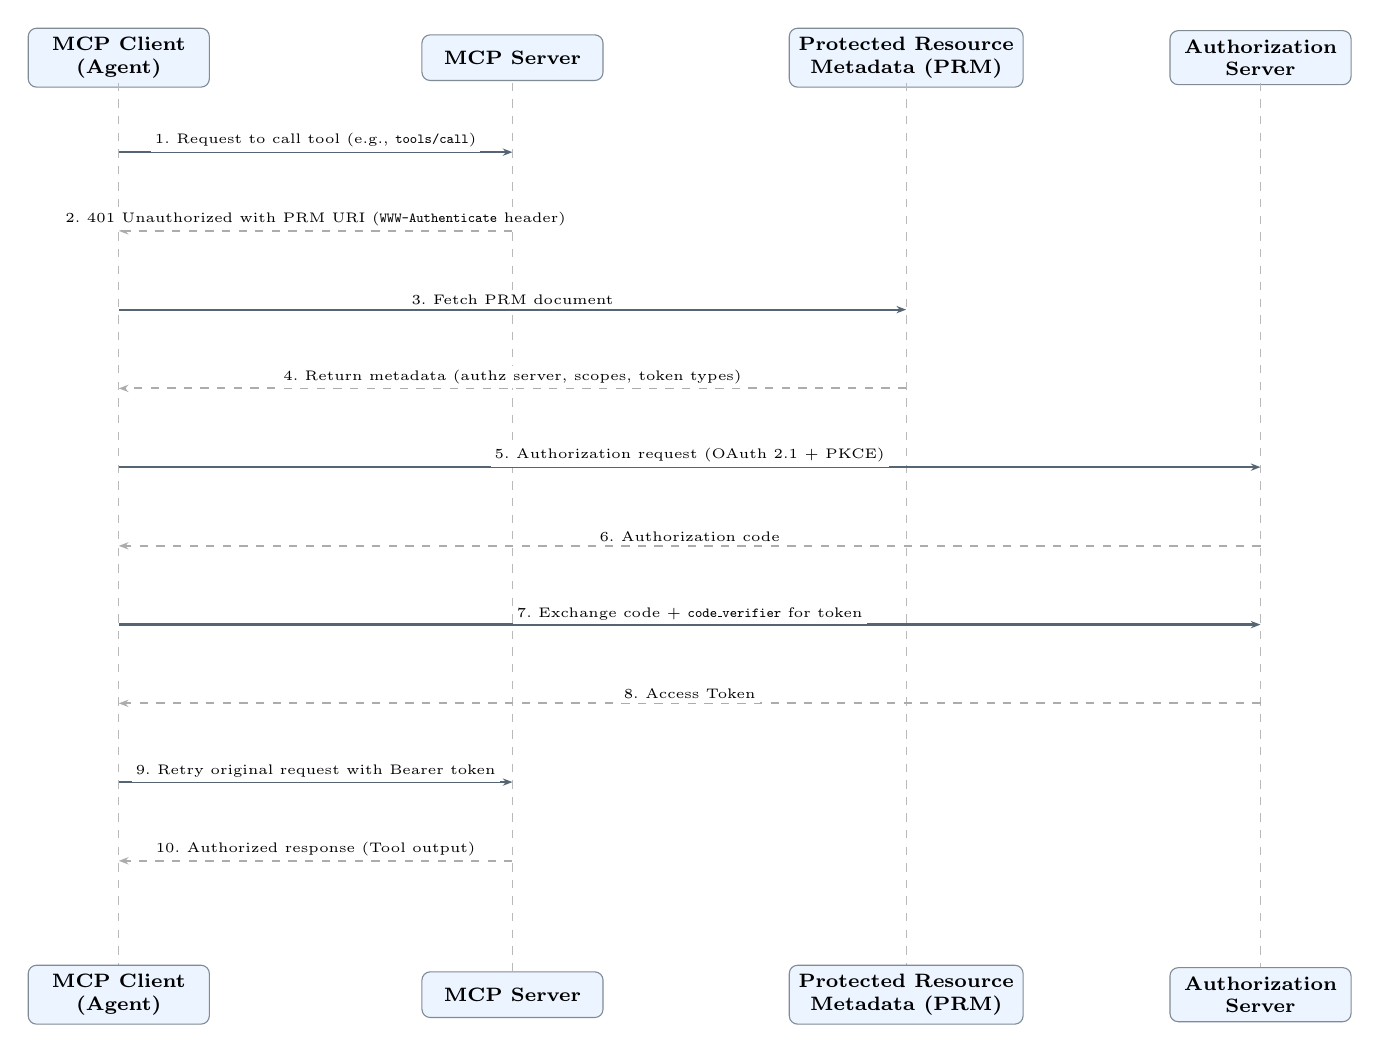
\begin{tikzpicture}[
  every node/.style={font=\scriptsize},
  x=1cm, y=1cm,
]
%% ── Actor x-positions ────────────────────────────────────────
%% textwidth ≈ 17cm; 4 actors, each 2.4cm wide, centred as below
\pgfmathsetmacro{\xC}{1.8}   % MCP Client
\pgfmathsetmacro{\xS}{6.8}   % MCP Server
\pgfmathsetmacro{\xP}{11.8}  % PRM
\pgfmathsetmacro{\xA}{16.3}  % Auth Server

%% ── Top actor boxes ──────────────────────────────────────────
\node[SD/actor, minimum width=2.3cm] (C1) at (\xC, 0)
  {MCP Client\\(Agent)};
\node[SD/actor, minimum width=2.3cm] (S1) at (\xS, 0)
  {MCP Server};
\node[SD/actor, minimum width=2.8cm] (P1) at (\xP, 0)
  {Protected Resource\\Metadata (PRM)};
\node[SD/actor, minimum width=2.3cm] (A1) at (\xA, 0)
  {Authorization\\Server};

%% ── Lifelines ────────────────────────────────────────────────
\draw[SD/life] (\xC,-0.32) -- (\xC,-11.6);
\draw[SD/life] (\xS,-0.32) -- (\xS,-11.6);
\draw[SD/life] (\xP,-0.32) -- (\xP,-11.6);
\draw[SD/life] (\xA,-0.32) -- (\xA,-11.6);

%% ── Messages ─────────────────────────────────────────────────
%% 1. Client → Server  (solid)
\draw[SD/fwd] (\xC,-1.2) -- (\xS,-1.2);
\node[SD/lbl, above] at ({(\xC+\xS)/2},-1.2)
  {1.\ Request to call tool (e.g., \texttt{tools/call})};

%% 2. Server → Client  (dashed, 401)
\draw[SD/bck] (\xS,-2.2) -- (\xC,-2.2);
\node[SD/lbl, above] at ({(\xC+\xS)/2},-2.2)
  {2.\ 401 Unauthorized with PRM URI (\texttt{WWW-Authenticate} header)};

%% 3. Client → PRM  (solid)
\draw[SD/fwd] (\xC,-3.2) -- (\xP,-3.2);
\node[SD/lbl, above] at ({(\xC+\xP)/2},-3.2)
  {3.\ Fetch PRM document};

%% 4. PRM → Client  (dashed)
\draw[SD/bck] (\xP,-4.2) -- (\xC,-4.2);
\node[SD/lbl, above] at ({(\xC+\xP)/2},-4.2)
  {4.\ Return metadata (authz server, scopes, token types)};

%% 5. Client → Auth  (solid)
\draw[SD/fwd] (\xC,-5.2) -- (\xA,-5.2);
\node[SD/lbl, above] at ({(\xC+\xA)/2},-5.2)
  {5.\ Authorization request (OAuth 2.1 + PKCE)};

%% 6. Auth → Client  (dashed)
\draw[SD/bck] (\xA,-6.2) -- (\xC,-6.2);
\node[SD/lbl, above] at ({(\xC+\xA)/2},-6.2)
  {6.\ Authorization code};

%% 7. Client → Auth  (solid)
\draw[SD/fwd] (\xC,-7.2) -- (\xA,-7.2);
\node[SD/lbl, above] at ({(\xC+\xA)/2},-7.2)
  {7.\ Exchange code + \texttt{code\_verifier} for token};

%% 8. Auth → Client  (dashed)
\draw[SD/bck] (\xA,-8.2) -- (\xC,-8.2);
\node[SD/lbl, above] at ({(\xC+\xA)/2},-8.2)
  {8.\ Access Token};

%% 9. Client → Server  (solid)
\draw[SD/fwd] (\xC,-9.2) -- (\xS,-9.2);
\node[SD/lbl, above] at ({(\xC+\xS)/2},-9.2)
  {9.\ Retry original request with Bearer token};

%% 10. Server → Client  (dashed)
\draw[SD/bck] (\xS,-10.2) -- (\xC,-10.2);
\node[SD/lbl, above] at ({(\xC+\xS)/2},-10.2)
  {10.\ Authorized response (Tool output)};

%% ── Bottom actor boxes (UML convention) ──────────────────────
\node[SD/actor, minimum width=2.3cm] at (\xC,-11.9)
  {MCP Client\\(Agent)};
\node[SD/actor, minimum width=2.3cm] at (\xS,-11.9)
  {MCP Server};
\node[SD/actor, minimum width=2.8cm] at (\xP,-11.9)
  {Protected Resource\\Metadata (PRM)};
\node[SD/actor, minimum width=2.3cm] at (\xA,-11.9)
  {Authorization\\Server};

\end{tikzpicture}
\caption{Standard MCP OAuth 2.1 + PKCE authorization flow (UML sequence
diagram). The MCP client discovers the authorization server via Protected
Resource Metadata, performs the OAuth 2.1 PKCE authorization code flow, and
obtains an access token. Solid arrows are requests; dashed arrows are
responses. Critically, \textbf{this flow covers only the client-to-hub
authorization boundary}. How the hub authorizes its own calls to downstream
worker services is unspecified---the delegation security gap this paper
addresses.}
\label{fig:mcp_std_auth}
\end{figure*}

%% ============================================================

\subsection{LLM Agents and the ReAct Model}

Modern LLMs exhibit emergent tool-use capabilities. In the \textit{ReAct}
paradigm \cite{yao2022react}, the model interleaves reasoning with action
calls: it selects a tool, calls it, observes the result, and re-plans. This
is the computational model underlying MCP tool use \cite{wang2024survey}.

\subsection{The Model Context Protocol}

MCP \cite{mcp_spec} defines a client-server protocol over JSON-RPC 2.0. An
\textit{MCP server} exposes \textit{tools} (callable functions), \textit{resources}
(data), and \textit{prompts} (templates) to an \textit{MCP client}. Authentication
is carried via the \texttt{Authorization: Bearer} HTTP header.

The MCP authorization specification \cite{mcp_spec_2025} treats MCP servers as
OAuth 2.1 resource servers. Figure~\ref{fig:mcp_std_auth} shows the standard
authorization flow: the MCP client discovers the authorization server via
Protected Resource Metadata (PRM), performs an OAuth 2.1 authorization code flow
with PKCE, obtains an access token, and uses it to call the MCP server. This flow
governs the \textit{client-to-hub} boundary only. It does not specify how the hub
should authorize its own calls to downstream worker services---the gap this paper
fills.

In multi-service deployments, the AI assistant hub acts as both an MCP server
(receiving tool calls from the agent) and an HTTP client (calling downstream
worker services). This dual role is the hub-and-spoke topology that the MCP
security specification identifies as the confused deputy attack surface.

\subsection{OAuth 2.1 and Bearer Tokens}

OAuth 2.1 \cite{oauth21} is the current revision of the OAuth 2.0 authorization
framework \cite{rfc6749}, mandating PKCE for all public clients and deprecating
the implicit grant. An \textit{access token} is a bearer credential encoding the
authorized subject (\texttt{sub}), audience (\texttt{aud}), and permission set
(\texttt{scope}).

RFC 9068 \cite{rfc9068} profiles access tokens as signed JSON Web Tokens
(JWTs) \cite{rfc7519}, enabling compact, cryptographically verifiable
credential exchange. Four JWT claims are central to this paper.
The \textbf{\texttt{aud}} claim identifies the intended recipient; a receiver
MUST reject tokens not addressed to it \cite{rfc9068}.
The \textbf{\texttt{scope}} claim carries the set of permissions the token grants.
The \textbf{\texttt{jti}} claim provides a unique per-token identifier that
enables single-use enforcement and replay prevention.
Finally, the \textbf{\texttt{act}} claim (defined by RFC 8693) records the
identity of the party exercising delegated authority, forming a verifiable
delegation chain.

\subsection{RFC 8693: OAuth 2.0 Token Exchange}

RFC 8693 \cite{rfc8693} defines an HTTP Security Token Service (STS) protocol
for exchanging one token for another with different properties.
We use the \textit{delegation} semantics: the acting party remains
distinguishable from the subject; the new token preserves \texttt{sub} = $u$
while recording the hub in a nested \texttt{act} claim. RFC 8693 also defines
the \textit{scope non-escalation invariant}: a derived token's scope must not
exceed the subject token's scope---the formal basis for P2. Token exchange endpoints compatible with the specification are available in
Microsoft Entra (OBO), Auth0, ZITADEL, Authlete, Keycloak, and Salesforce
\cite{rfc8693_deploy}.

\subsection{JTI State Stores}

RFC 7009 \cite{rfc7009} motivates OAuth 2.0 token revocation semantics. Our
reference implementation uses a separate JTI state store to enforce atomic
single-use consumption, extending the revocation concept to per-request
granularity. The canonical architecture is an in-memory key-value store
with TTL-based expiry: the identifier is written on issuance
(\textit{register}) and \textit{atomically consumed} on first presentation---a
single store operation that checks the identifier's status and marks it as
spent, preventing concurrent replay.  Any implementation supporting atomic
check-and-set with TTL-based expiry---whether managed (e.g., AWS ElastiCache,
Google Memorystore) or self-hosted (e.g., Redis with Lua scripts,
DragonflyDB)---satisfies the requirement. The specific technology choice
affects operational latency and availability, not security semantics.

\subsection{OWASP Generative AI Top 10 (2025)}

The OWASP Top 10 for Large Language Model Applications 2025 \cite{owasp_genai}
identifies the most critical LLM security risks. Two entries are directly
relevant to this work. \textbf{LLM06:2025 Excessive Agency} arises when agents
are granted more permissions or capability than their task requires---this is the
root cause of the scope escalation attack vector studied in this paper.
\textbf{LLM01:2025 Prompt Injection} describes attacker-controlled input that
causes an agent to exercise legitimately authorized tokens in unauthorised ways,
an effect that is significantly amplified when tokens carry excess scopes.


%% ============================================================
\section{Problem Statement}
\label{sec:problem}
%% ============================================================

\subsection{The Token Passthrough Anti-Pattern}

Let $\mathcal{H}$ denote the assistant hub, $\mathcal{W}=\{W_1,\ldots,W_n\}$ the
set of downstream worker services, $u$ the authenticated user, and $\mathcal{A}$
the OAuth authorization server. $\mathcal{A}$ issues a root access token:

\begin{equation}
T_0 = \mathrm{JWT}\!\left(\begin{array}{l}
  \texttt{sub} = u,\quad \texttt{aud} = \mathcal{H},\\[2pt]
  \texttt{scope} = S_0 = \textstyle\bigcup_{i}\, s_i,\quad
  \texttt{jti} = j_0
\end{array}\right)
\label{eq:root}
\end{equation}

where $S_0$ is the union of all scopes required by any worker. In the token
passthrough pattern, $\mathcal{H}$ forwards $T_0$ unchanged to every worker:

\begin{equation}
\mathrm{call}(W_i,\; T_0) \quad \forall\, i \in \{1, \ldots, n\}
\label{eq:passthrough}
\end{equation}

Figure~\ref{fig:passthrough} visualises this topology.

%%  --- FIGURE 2: Token Passthrough Architecture ----
\begin{figure}[t]
\centering
\resizebox{\columnwidth}{!}{%
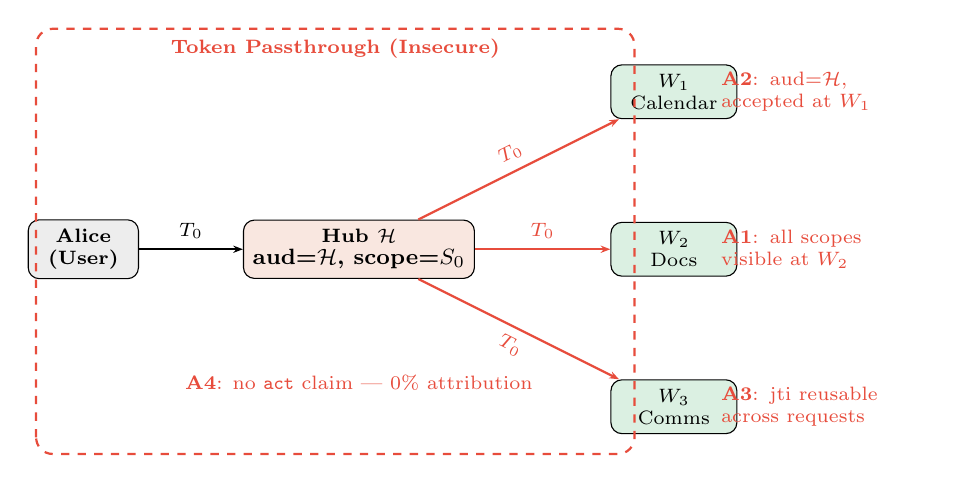
\begin{tikzpicture}[
  every node/.style={font=\small},
  x=1cm, y=1cm,
]
%% Nodes
\node[arch/user]  (alice) at (0, 2.5)   {Alice\\(User)};
\node[arch/oauth] (hub)   at (3.5, 2.5)
  {Hub $\mathcal{H}$\\{\footnotesize aud=$\mathcal{H}$, scope=$S_0$}};
\node[arch/worker](w1)    at (7.5, 4.5)  {$W_1$\\Calendar};
\node[arch/worker](w2)    at (7.5, 2.5)  {$W_2$\\Docs};
\node[arch/worker](w3)    at (7.5, 0.5)  {$W_3$\\Comms};

%% Alice → Hub
\draw[arch/arr] (alice) -- node[above,font=\scriptsize]{$T_0$} (hub);

%% Hub → Workers (same token)
\draw[arch/arr, color=C_WARN]
  (hub) -- node[above,sloped,font=\scriptsize]{$T_0$} (w1);
\draw[arch/arr, color=C_WARN]
  (hub) -- node[above,font=\scriptsize]{$T_0$} (w2);
\draw[arch/arr, color=C_WARN]
  (hub) -- node[below,sloped,font=\scriptsize]{$T_0$} (w3);

%% Attack annotations (below each arrow, right side)
\node[font=\scriptsize, color=C_WARN, text width=2.6cm, align=left]
  at (9.4, 4.5)
  {\textbf{A2}: aud=$\mathcal{H}$,\\accepted at $W_1$};
\node[font=\scriptsize, color=C_WARN, text width=2.6cm, align=left]
  at (9.4, 2.5)
  {\textbf{A1}: all scopes\\visible at $W_2$};
\node[font=\scriptsize, color=C_WARN, text width=2.6cm, align=left]
  at (9.4, 0.5)
  {\textbf{A3}: jti reusable\\across requests};

%% A4 annotation under hub
\node[font=\scriptsize, color=C_WARN, align=center]
  at (3.5, 0.8)
  {\textbf{A4}: no \texttt{act} claim — 0\% attribution};

%% Border box indicating vulnerability
\draw[draw=C_WARN, dashed, thick, rounded corners=6pt]
  (-0.6, -0.1) rectangle (7.0, 5.3);
\node[font=\scriptsize\bfseries, color=C_WARN] at (3.2, 5.05)
  {Token Passthrough (Insecure)};
\end{tikzpicture}
}
\caption{Token passthrough anti-pattern: the hub forwards $T_0$ (with
hub-bound audience and full scope $S_0$) \emph{unchanged} to every worker,
simultaneously enabling all four attacks (A1--A4) \cite{mcp_security,cosai_mcp}.}
\label{fig:passthrough}
\end{figure}

\subsection{Three Violated Security Properties}

\begin{definition}[\textbf{Audience Binding, P1}]
A token $T$ satisfies audience binding for worker $W_i$ iff
$\mathrm{aud}(T) = \mathrm{AUDIENCE}(W_i)$.
\end{definition}

\textbf{Violation:} $T_0$ carries $\texttt{aud} = \mathcal{H}$. When presented
to $W_i \neq \mathcal{H}$, RFC~9068 requires rejection. In practice, many
implementations omit this check.

\begin{definition}[\textbf{Scope Attenuation, P2}]
A token $T$ satisfies scope attenuation for $W_i$ iff
$\mathrm{scope}(T) \subseteq s_i$, where $s_i$ is the minimum scope $W_i$
requires to execute its function.
\end{definition}

\textbf{Violation:} $T_0$ carries the union of all service scopes,
$S_0 = \bigcup_j s_j$. Each worker therefore receives permissions intended
for every other service, violating the principle of least privilege. A
compromised worker inherits the full authority of the entire system.

\begin{definition}[\textbf{Delegation Chain Visibility, P3}]
A token $T$ satisfies chain visibility iff the \texttt{act} claim of $T$
contains a cryptographically verifiable record of \emph{every} agent that
handled $T$ on behalf of subject $u$ (complete chain, all hops), not merely
the immediate actor.
\end{definition}

\textbf{Violation:} $T_0$ carries no \texttt{act} claim. Every audit record
contains only $\texttt{sub} = u$. Calls originating from different agents are
indistinguishable in the audit trail.

\subsection{The Confused Deputy Problem in MCP}

Hardy's 1988 analysis \cite{hardy1988} applies directly. The \textbf{principal}
is user $u$, who delegated authority $T_0$ to $\mathcal{H}$. The \textbf{deputy}
is hub $\mathcal{H}$, which holds $T_0$ and calls workers on the user's behalf.
The \textbf{confused action} occurs when $\mathcal{H}$ presents $T_0$ to
worker $W_i$, where it carries capabilities that $u$ never intended for $W_i$.
The \textbf{adversary} is any agent or prompt injection payload that exploits
the excess authority embedded in $T_0$.

The MCP specification \cite{mcp_security} states: ``Servers SHOULD NOT pass
tokens received from clients to other servers, as this creates confused deputy
risks.''

\subsection{Four Concrete Attack Vectors}

Table~\ref{tab:attack_formal} formally defines the four attack vectors that arise from P1--P3 violations.

\begin{table}[h]
\caption{Formal attack vector definitions. Each attack exploits the absence of
one or more security properties (P1~=~audience binding, P2~=~scope attenuation,
P3~=~delegation chain visibility). The ``Requires'' column identifies which
property must be absent for the attack to succeed.}
\label{tab:attack_formal}
\centering
\footnotesize
\setlength{\tabcolsep}{3pt}
\begin{tabularx}{\columnwidth}{l X c}
\toprule
\textbf{ID} & \textbf{Mechanism} & \textbf{Requires} \\
\midrule
A1 & Agent calls a privileged tool using a token without the required scope
     & $\neg$\,P2 \\
A2 & Token obtained for service $W_i$ is replayed at $W_j\;(i\neq j)$
     & $\neg$\,P1 \\
A3 & Captured child token is replayed for a second unauthorised call
     & No single-use enforcement \\
A4 & Audit log lacks delegation chain; calls cannot be attributed to agent
     & $\neg$\,P3 \\
\bottomrule
\end{tabularx}
\end{table}


%% ============================================================
\section{The RFC 8693 NAC Architectural Pattern}
\label{sec:solution}
%% ============================================================

%% ---- FIGURE 5: Side-by-side sequence comparison (full width) ----
%% Placed at the very top of the section per IEEEtran float rules.
%% Left panel: token passthrough (insecure baseline).
%% Right panel: RFC 8693 NAC (secure pattern).
\begin{figure*}[!t]
\centering
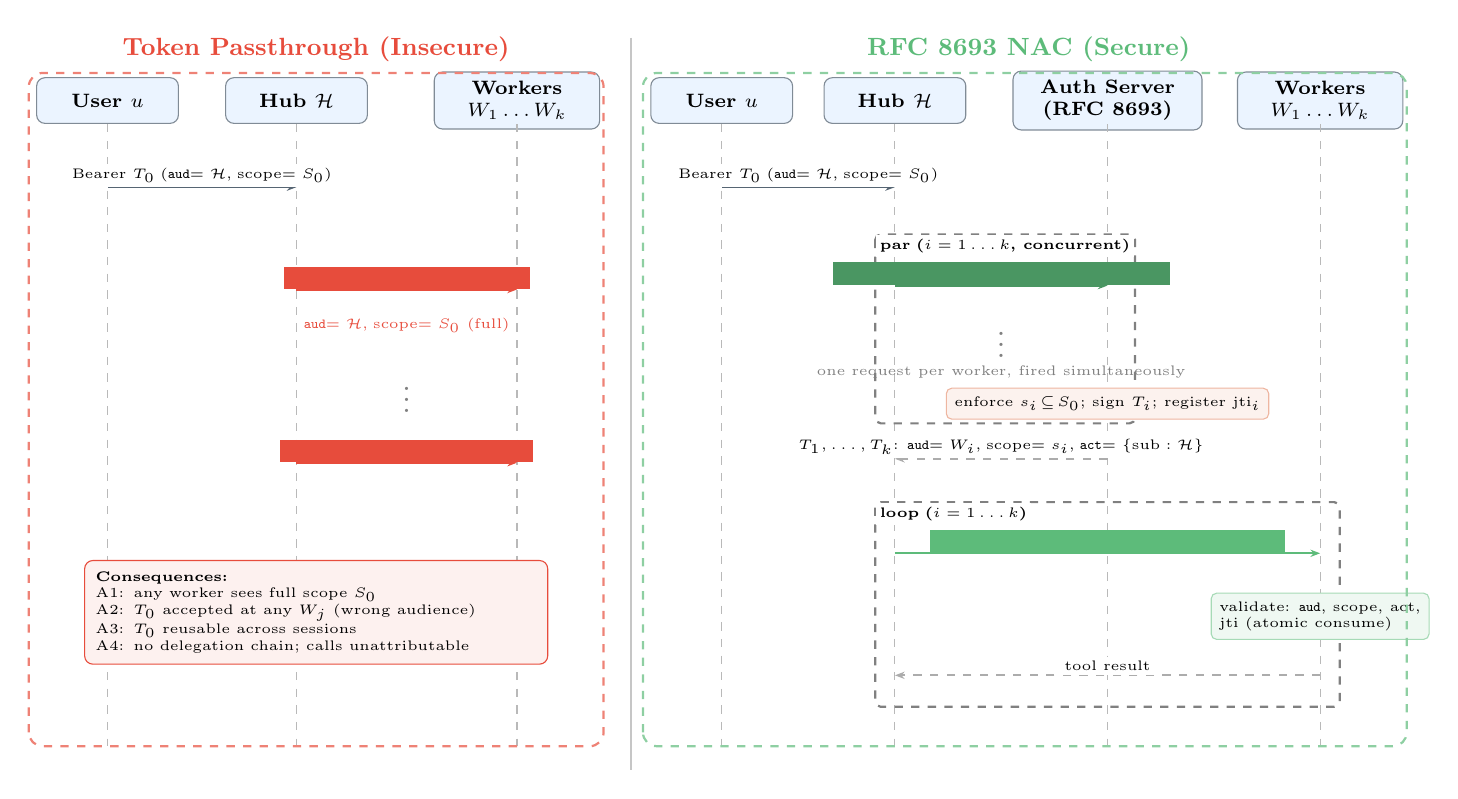
\begin{tikzpicture}[
  every node/.style={font=\scriptsize},
  x=1cm, y=1cm,
]

%% ━━━━━━━━━━━━━━━━━━━━━━━━━━━━━━━━━━━━━━━━━━━━━━━━━━━━━━━━━━━━━━━━━━━━━
%%  LEFT PANEL — Token Passthrough (Insecure Baseline)
%% ━━━━━━━━━━━━━━━━━━━━━━━━━━━━━━━━━━━━━━━━━━━━━━━━━━━━━━━━━━━━━━━━━━━━━
\pgfmathsetmacro{\lxU}{1.0}  %% User
\pgfmathsetmacro{\lxH}{3.4}  %% Hub
\pgfmathsetmacro{\lxW}{6.2}  %% Workers (W_1 … W_k combined)

%% Panel title
\node[font=\small\bfseries, color=C_WARN] at (3.65, 0.65)
  {Token Passthrough (Insecure)};

%% Actor boxes
\node[SD/actor, minimum width=1.8cm] at (\lxU,0) {User $u$};
\node[SD/actor, minimum width=1.8cm] at (\lxH,0) {Hub $\mathcal{H}$};
\node[SD/actor, minimum width=2.1cm] at (\lxW,0)
  {Workers\\$W_1 \ldots W_k$};

%% Lifelines
\draw[SD/life] (\lxU,-0.30) -- (\lxU,-8.2);
\draw[SD/life] (\lxH,-0.30) -- (\lxH,-8.2);
\draw[SD/life] (\lxW,-0.30) -- (\lxW,-8.2);

%% 1. User → Hub: root token T0
\draw[SD/fwd] (\lxU,-1.1) -- (\lxH,-1.1);
\node[SD/lbl, above] at ({(\lxU+\lxH)/2},-1.1)
  {Bearer $T_0$\;(\texttt{aud}$=\mathcal{H}$,\;scope$=S_0$)};

%% 2. Hub → Workers: same T0 forwarded unchanged (first worker)
\draw[SD/fwd, color=C_WARN, thick] (\lxH,-2.4) -- (\lxW,-2.4);
\node[SD/lbl, above, color=C_WARN] at ({(\lxH+\lxW)/2},-2.4)
  {$T_0$ unchanged \textemdash{} all workers};
\node[font=\tiny, color=C_WARN, align=center]
  at ({(\lxH+\lxW)/2},-2.85)
  {\texttt{aud}$=\mathcal{H}$,\;scope$=S_0$ (full)};

%% Vertical dots (represents repeated passthrough to each worker)
\node[font=\large, color=gray] at ({(\lxH+\lxW)/2},-3.7) {$\vdots$};

%% 3. Hub → Workers: same T0 (k-th call)
\draw[SD/fwd, color=C_WARN, thick] (\lxH,-4.6) -- (\lxW,-4.6);
\node[SD/lbl, above, color=C_WARN] at ({(\lxH+\lxW)/2},-4.6)
  {$T_0$ unchanged \textemdash{} $k$-th worker};

%% Attack consequence box
\node[draw=C_WARN, fill=C_WARN!8, rounded corners=3pt,
      font=\tiny, align=left, inner sep=4pt, text width=5.6cm]
  at (3.65,-6.5)
  {\textbf{Consequences:}\\
   A1: any worker sees full scope $S_0$\\
   A2: $T_0$ accepted at any $W_j$ (wrong audience)\\
   A3: $T_0$ reusable across sessions\\
   A4: no delegation chain; calls unattributable};

%% Left panel border
\draw[draw=C_WARN!70, dashed, thick, rounded corners=5pt]
  (0.0,-8.2) rectangle (7.3,0.35);

%% ━━━━━━━━━━━━━━━━━━━━━━━━━━━━━━━━━━━━━━━━━━━━━━━━━━━━━━━━━━━━━━━━━━━━━
%%  VERTICAL DIVIDER
%% ━━━━━━━━━━━━━━━━━━━━━━━━━━━━━━━━━━━━━━━━━━━━━━━━━━━━━━━━━━━━━━━━━━━━━
\draw[thick, gray!45] (7.65, 0.8) -- (7.65,-8.5);

%% ━━━━━━━━━━━━━━━━━━━━━━━━━━━━━━━━━━━━━━━━━━━━━━━━━━━━━━━━━━━━━━━━━━━━━
%%  RIGHT PANEL — RFC 8693 NAC (Secure Pattern)
%% ━━━━━━━━━━━━━━━━━━━━━━━━━━━━━━━━━━━━━━━━━━━━━━━━━━━━━━━━━━━━━━━━━━━━━
\pgfmathsetmacro{\rxU}{8.8}   %% User
\pgfmathsetmacro{\rxH}{11.0}  %% Hub
\pgfmathsetmacro{\rxA}{13.7}  %% Auth Server
\pgfmathsetmacro{\rxW}{16.4}  %% Workers

%% Panel title
\node[font=\small\bfseries, color=C_PAR] at (12.7, 0.65)
  {RFC 8693 NAC (Secure)};

%% Actor boxes
\node[SD/actor, minimum width=1.8cm] at (\rxU,0) {User $u$};
\node[SD/actor, minimum width=1.8cm] at (\rxH,0) {Hub $\mathcal{H}$};
\node[SD/actor, minimum width=2.4cm] at (\rxA,0)
  {Auth Server\\(RFC 8693)};
\node[SD/actor, minimum width=2.1cm] at (\rxW,0)
  {Workers\\$W_1 \ldots W_k$};

%% Lifelines
\draw[SD/life] (\rxU,-0.30) -- (\rxU,-8.2);
\draw[SD/life] (\rxH,-0.30) -- (\rxH,-8.2);
\draw[SD/life] (\rxA,-0.30) -- (\rxA,-8.2);
\draw[SD/life] (\rxW,-0.30) -- (\rxW,-8.2);

%% 1. User → Hub: root token T0
\draw[SD/fwd] (\rxU,-1.1) -- (\rxH,-1.1);
\node[SD/lbl, above] at ({(\rxU+\rxH)/2},-1.1)
  {Bearer $T_0$\;(\texttt{aud}$=\mathcal{H}$,\;scope$=S_0$)};

%% 2. Concurrent exchange — "par" combined fragment
\draw[SD/par] (\rxH-0.25,-1.7) rectangle (\rxA+0.35,-4.1);
\node[font=\tiny\bfseries, fill=white, inner sep=1.5pt, anchor=north west]
  at (\rxH-0.25,-1.7) {par\;($i = 1\ldots k$, concurrent)};

%% Hub → Auth: exchange request (per worker)
\draw[SD/fwd, color=C_PAR!80!black] (\rxH,-2.35) -- (\rxA,-2.35);
\node[SD/lbl, above, color=C_PAR!80!black] at ({(\rxH+\rxA)/2},-2.35)
  {\texttt{POST /token/exchange}\;(\texttt{aud}$=W_i$,\;scope$=s_i$)};

\node[font=\large, color=gray] at ({(\rxH+\rxA)/2},-3.0) {$\vdots$};
\node[font=\tiny, color=gray, align=center]
  at ({(\rxH+\rxA)/2},-3.45) {one request per worker, fired simultaneously};

%% Auth Server: validates, signs child tokens
\node[draw=C_BASE!55, fill=C_BASE!10, rounded corners=2pt,
      font=\tiny, align=center, inner sep=3pt]
  at (\rxA,-3.85)
  {enforce $s_i \!\subseteq\! S_0$; sign $T_i$; register jti$_i$};

%% Auth → Hub: child tokens returned
\draw[SD/bck] (\rxA,-4.55) -- (\rxH,-4.55);
\node[SD/lbl, above] at ({(\rxH+\rxA)/2},-4.55)
  {$T_1,\ldots,T_k$: \texttt{aud}$=W_i$,\;scope$=s_i$,\;\texttt{act}$=\{\text{sub}:\mathcal{H}\}$};

%% 3. Worker invocation — "loop" combined fragment
\draw[SD/par] (\rxH-0.25,-5.1) rectangle (\rxW+0.25,-7.7);
\node[font=\tiny\bfseries, fill=white, inner sep=1.5pt, anchor=north west]
  at (\rxH-0.25,-5.1) {loop\;($i = 1\ldots k$)};

%% Hub → Workers: Ti (unique per worker)
\draw[SD/fwd, color=C_PAR] (\rxH,-5.75) -- (\rxW,-5.75);
\node[SD/lbl, above, color=C_PAR] at ({(\rxH+\rxW)/2},-5.75)
  {Bearer $T_i$\;(\texttt{aud}$=W_i$,\;scope$=s_i$,\;\texttt{act} chain)};

%% Worker validation annotation
\node[draw=C_PAR!55, fill=C_PAR!10, rounded corners=2pt,
      font=\tiny, align=left, inner sep=3pt]
  at (\rxW,-6.55)
  {validate: \texttt{aud}, scope, act,\\jti (atomic consume)};

%% Workers → Hub: tool result
\draw[SD/bck] (\rxW,-7.3) -- (\rxH,-7.3);
\node[SD/lbl, above] at ({(\rxH+\rxW)/2},-7.3) {tool result};

%% Right panel border
\draw[draw=C_PAR!70, dashed, thick, rounded corners=5pt]
  (7.8,-8.2) rectangle (17.5,0.35);

\end{tikzpicture}
\caption{Side-by-side sequence comparison of token passthrough (left) and the
RFC~8693 NAC pattern (right). In the baseline flow, the hub forwards the
unchanged root token $T_0$ to all workers, simultaneously exposing attacks
A1--A4. In the NAC flow, the hub exchanges $T_0$ for $k$ per-service child
tokens at the authorization server (concurrent, \textit{par} fragment) before
invoking any worker; each child token carries a unique audience, an attenuated
scope, a verifiable \texttt{act} chain, and a one-time-use \texttt{jti},
blocking all four attacks by construction.}
\label{fig:seq_comparison}
\end{figure*}

\subsection{Pattern Overview}

Figure~\ref{fig:seq_comparison} contrasts the two flows at a glance.
Before invoking worker $W_i$, the orchestrating hub presents its current token
to the authorization server's token exchange endpoint and obtains a fresh,
narrowly scoped child token:

\begin{equation}
T_i = \mathrm{Exchange}\!\left(
  T_{\mathrm{parent}},\;
  \mathrm{AUDIENCE}(W_i),\;
  s_i,\;
  \mathcal{H}
\right)
\label{eq:exchange}
\end{equation}

where $T_i$ is constructed by the authorization server as:

\begin{equation}
T_i = \mathrm{JWT}\!\left(\begin{array}{l}
  \texttt{sub} = u, \\[2pt]
  \texttt{aud} = \mathrm{AUDIENCE}(W_i), \\[2pt]
  \texttt{scope} = s_i \;\subseteq\; \mathrm{scope}(T_{\mathrm{parent}}), \\[2pt]
  \texttt{jti} = j_i \;\text{(fresh, unique)}, \\[2pt]
  \texttt{act} = \{\,\texttt{sub}\text{:}\,\mathcal{H},\;
                    \texttt{act}\text{:}\,T_{\mathrm{parent}}.\texttt{act}\,\}
\end{array}\right)
\label{eq:child}
\end{equation}

This construction directly restores all three violated properties: the
\texttt{aud} satisfies P1, the scope satisfies P2, and the \texttt{act} chain
satisfies P3. Figure~\ref{fig:nac_arch} shows the NAC architecture, and
Figure~\ref{fig:nac_seq} illustrates the complete token exchange sequence.

Listing~\ref{lst:child} shows the reference implementation's child token
payload construction, which maps directly to Equation~(\ref{eq:child}).

\begin{lstlisting}[language=Python, label=lst:child,
  caption={Child token construction (\texttt{nac\_common.py}).
  Each field enforces one security property.}]
payload = {
  "sub":   parent["sub"],        # preserved
  "aud":   new_audience,         # P1
  "scope": scope_str(new_scope), # P2
  "jti":   str(uuid.uuid4()),   # P4
  "act":   {"sub": actor,        # P3
    "act": parent.get("act")},
}
token = jwt.encode(payload, key, "RS256")
\end{lstlisting}

%% ---- FIGURE 3: NAC Architecture (single column, fixed) ----
\begin{figure}[t]
\centering
\resizebox{\columnwidth}{!}{%
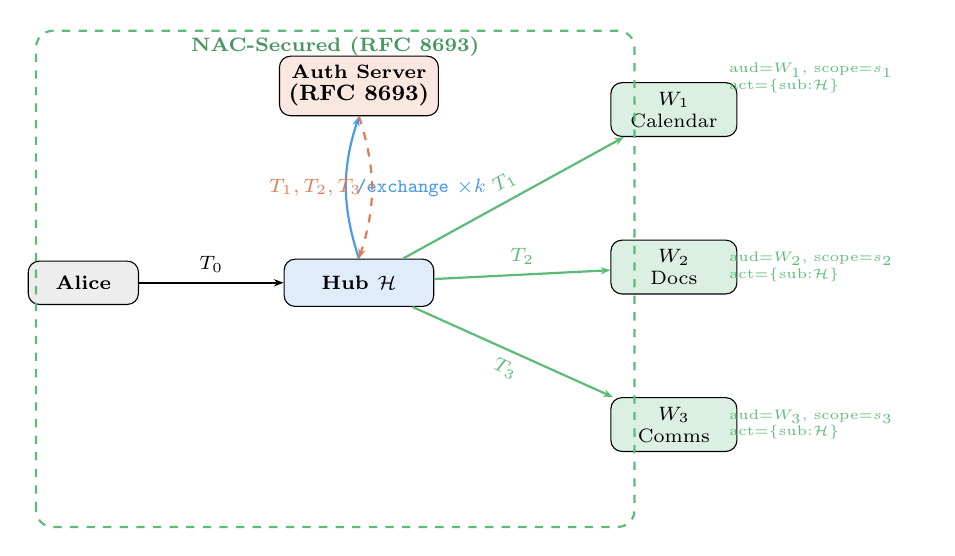
\begin{tikzpicture}[
  every node/.style={font=\small},
  x=1cm, y=1cm,
]
%% Nodes
\node[arch/user]  (alice)  at (0, 3.0)
  {Alice};
\node[arch/oauth] (auth)   at (3.5, 5.5)
  {Auth Server\\{\footnotesize(RFC 8693)}};
\node[arch/hub]   (hub)    at (3.5, 3.0)
  {Hub $\mathcal{H}$};
\node[arch/worker](w1)     at (7.5, 5.2)
  {$W_1$\\Calendar};
\node[arch/worker](w2)     at (7.5, 3.2)
  {$W_2$\\Docs};
\node[arch/worker](w3)     at (7.5, 1.2)
  {$W_3$\\Comms};

%% Alice → Hub
\draw[arch/arr] (alice) -- node[above,font=\scriptsize]{$T_0$} (hub);

%% Hub ↔ Auth Server (exchange)
\draw[arch/arr, color=C_SEC, bend left=18]
  (hub.north) to node[right,font=\scriptsize,pos=0.5]
    {\texttt{/exchange} $\times k$} (auth.south);
\draw[arch/darr, color=C_BASE, bend left=18]
  (auth.south) to node[left,font=\scriptsize,pos=0.5]
    {$T_1, T_2, T_3$} (hub.north);

%% Hub → Workers (different tokens, colour-coded)
\draw[arch/arr, color=C_PAR]
  (hub) -- node[above,sloped,font=\scriptsize]{$T_1$} (w1);
\draw[arch/arr, color=C_PAR]
  (hub) -- node[above,font=\scriptsize]{$T_2$} (w2);
\draw[arch/arr, color=C_PAR]
  (hub) -- node[below,sloped,font=\scriptsize]{$T_3$} (w3);

%% Token property labels next to workers
\node[font=\tiny, color=C_PAR, text width=2.4cm, align=left]
  at (9.4, 5.6)
  {aud=$W_1$, scope=$s_1$\\act=\{sub:$\mathcal{H}$\}};
\node[font=\tiny, color=C_PAR, text width=2.4cm, align=left]
  at (9.4, 3.2)
  {aud=$W_2$, scope=$s_2$\\act=\{sub:$\mathcal{H}$\}};
\node[font=\tiny, color=C_PAR, text width=2.4cm, align=left]
  at (9.4, 1.2)
  {aud=$W_3$, scope=$s_3$\\act=\{sub:$\mathcal{H}$\}};

%% Green border indicating security
\draw[draw=C_PAR, dashed, thick, rounded corners=6pt]
  (-0.6, -0.1) rectangle (7.0, 6.2);
\node[font=\scriptsize\bfseries, color=C_PAR!80!black]
  at (3.2, 6.0) {NAC-Secured (RFC 8693)};
\end{tikzpicture}
}
\caption{RFC 8693 NAC pattern: the hub exchanges the root token $T_0$ for
per-service child tokens at the authorization server before each worker call.
Each $T_i$ carries a unique \texttt{aud}, attenuated \texttt{scope}, and
nested \texttt{act} chain, satisfying P1--P3 simultaneously.}
\label{fig:nac_arch}
\end{figure}

\subsection{Concurrent Issuance for Multiple Workers}

Because child tokens for $W_1, W_2, \ldots, W_k$ are issued from the same parent
token and are mutually independent (different audience, different scope, no
ordering constraint), they can be issued concurrently:

\begin{multline}
(T_1, T_2, \ldots, T_k) = \\
\mathrm{ConcurrentExchange}\!\left(
  T_{\mathrm{root}},\;
  \bigl\{\,(\mathrm{aud}_i,\; s_i)\,\bigr\}_{i=1}^{k}
\right)
\label{eq:concurrent}
\end{multline}

Concurrent issuance reduces wall-clock time from $k \times t_{\mathrm{exchange}}$
to $\approx t_{\mathrm{exchange}}$ (the maximum across concurrent requests),
subject to authorization server capacity. This is the basis for the
``parallel estimate'' in Section~\ref{sec:eval}.

\begin{proposition}[\textbf{Overhead Bound}]
\label{prop:overhead}
For $k$ independent workers, sequential NAC overhead is $O(k)$ with a
constant equal to one RSA signing operation plus one JTI store write
per hop. Under concurrent issuance with sufficient authorization-server parallelism,
wall-clock overhead is near-constant in $k$, bounded by
$t_{\mathrm{sign}} + t_{\mathrm{store}}$ --- the cost of a single
exchange --- regardless of how many workers are invoked.
\end{proposition}
\begin{proof}
Each child token exchange is a function solely of
$(T_{\mathrm{root}},\, \mathrm{aud}_i,\, s_i)$. Because no exchange reads or
modifies the output of any other exchange, the $k$ operations are fully
independent --- there is no cross-exchange data dependency. Sequential
execution therefore costs exactly $k \cdot (t_{\mathrm{sign}} +
t_{\mathrm{store}} + t_{\mathrm{http}})$; concurrent execution via
\texttt{asyncio.gather} or equivalent reduces the wall-clock component to
$\max_i(t_{\mathrm{exchange},i})$, which approaches $t_{\mathrm{sign}} +
t_{\mathrm{store}}$ when exchanges are dispatched simultaneously. The signing
and store operations are cryptographically fixed-cost (RSA-2048 sign,
sub-millisecond Redis write); only $t_{\mathrm{http}}$ varies with deployment
topology and is eliminable via co-location of the authorization server with
the hub.
\end{proof}

Listing~\ref{lst:gather} shows the hub implementation that realises
Equation~(\ref{eq:concurrent}) — all four RFC~8693 exchanges are dispatched
simultaneously via \texttt{asyncio.gather}, collapsing sequential latency
$k \times t_{\mathrm{exchange}}$ to a single round-trip.

\begin{lstlisting}[language=Python, label=lst:gather,
  caption={Concurrent RFC 8693 exchange (\texttt{assistant\_server.py});
  all four tokens are issued in parallel, achieving near-constant wall-clock
  overhead in $k$ workers.}]
tokens = await asyncio.gather(
  _get_token(root, "calendar", ["calendar:read"]),
  _get_token(root, "docs",     ["docs:read"]),
  _get_token(root, "comms",    ["email:send"]),
  _get_token(root, "comms",    ["slack:write"]),
)
cal, docs, email, slack = tokens
\end{lstlisting}

\subsection{N-Hop Delegation Chains}

For hierarchical delegation---where $W_i$ must itself call a further downstream
service---the pattern applies recursively:

\begin{equation}
T_k = \mathrm{Exchange}(T_{k-1},\;
  \mathrm{AUDIENCE}(W_k),\; s_k,\; W_{k-1})
\label{eq:nhop}
\end{equation}

The \texttt{act} claim grows by one level per hop, recording the complete
delegation history; the IETF Cross-Domain Attributes in Authentication and
Authorization Mechanisms (CAAM) draft \cite{ietf_caam} formalises this
multi-hop trust model. A depth limit prevents unbounded chain growth or
circular references. We demonstrate a 3-hop chain:
$\text{alice} \to \mathcal{H} \to W_{\mathrm{cal}} \to W_{\mathrm{ext}}$.

\subsection{NAC Token Exchange Sequence}

Figure~\ref{fig:nac_seq} provides the full UML sequence diagram for the NAC
token exchange flow. The diagram uses four actors---Alice, the hub
$\mathcal{H}$, the authorization server, and a representative worker
$W_i$---to show the general $k$-worker pattern. Phase~2 uses a ``par''
combined fragment for the concurrent exchanges; Phase~3 uses a ``loop''
fragment for the sequential worker invocations, each with its own
atomic validate-and-consume gate (P1--P4 checked before business logic runs).

%% ---- FIGURE 4: NAC Exchange Sequence Diagram (full width) ----
%% Redesigned: 4 actors (Alice, Hub, Auth Server, Worker Wi) with
%% proper spacing matching the reference MCP OAuth flow style.
%% Uses par fragment for concurrent exchanges, loop fragment for
%% worker calls, and activation boxes for worker validation steps.
\begin{figure*}[!t]
\centering
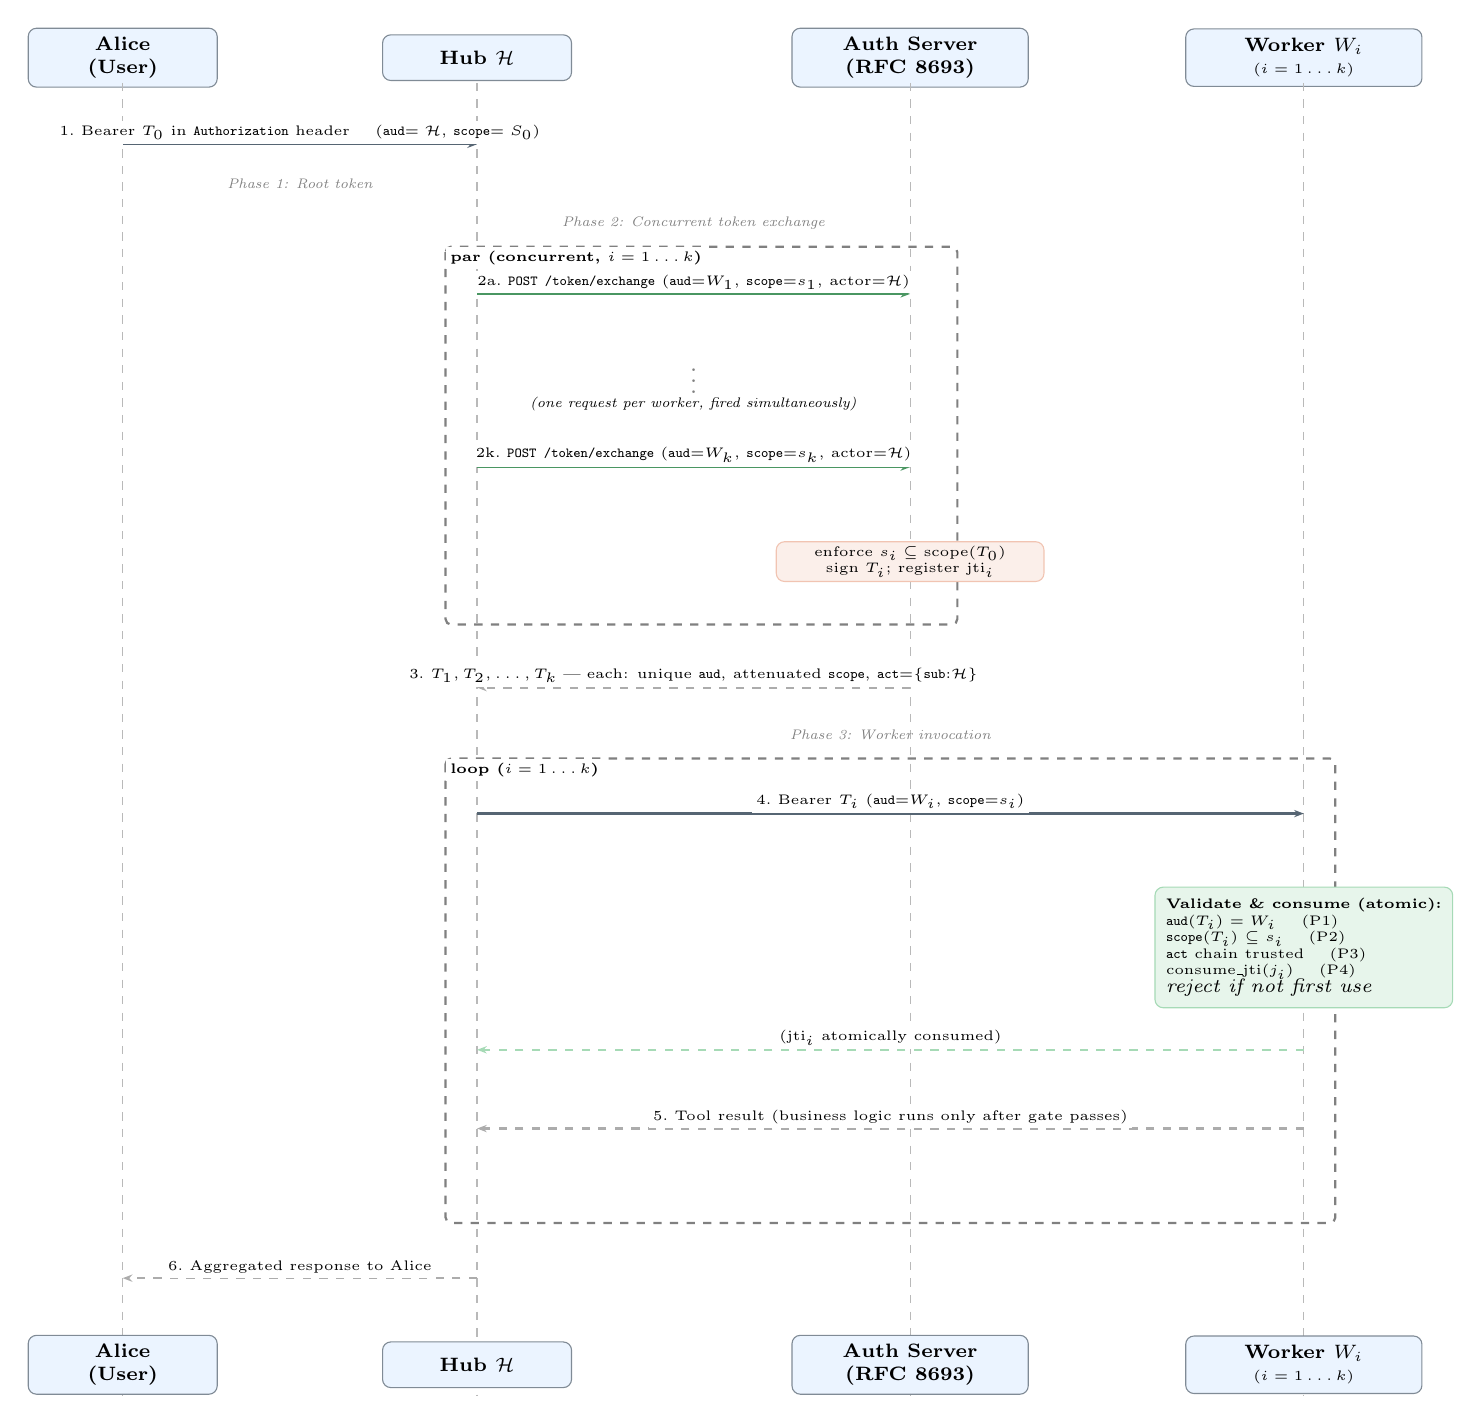
\begin{tikzpicture}[
  every node/.style={font=\scriptsize},
  x=1cm, y=1cm,
]

%% ── Actor x-positions ──────────────────────────────────────────────────────
%% 4 actors across ~17cm textwidth — matches the reference image spacing style
%% Each actor is ~2.6cm wide; gaps of ~4cm give clear, uncrossed lifelines.
\pgfmathsetmacro{\xAl}{1.5}   %% Alice (User)
\pgfmathsetmacro{\xHu}{6.0}   %% Hub H
\pgfmathsetmacro{\xAu}{11.5}  %% Auth Server (RFC 8693)
\pgfmathsetmacro{\xWk}{16.5}  %% Worker W_i  (represents all k workers)

%% ── Top actor boxes ────────────────────────────────────────────────────────
\node[SD/actor, minimum width=2.4cm] (A1) at (\xAl, 0)
  {Alice\\(User)};
\node[SD/actor, minimum width=2.4cm] (H1) at (\xHu, 0)
  {Hub $\mathcal{H}$};
\node[SD/actor, minimum width=3.0cm] (Au1) at (\xAu, 0)
  {Auth Server\\(RFC 8693)};
\node[SD/actor, minimum width=3.0cm] (W1) at (\xWk, 0)
  {Worker $W_i$\\{\tiny$(i = 1 \ldots k)$}};

%% ── Lifelines ──────────────────────────────────────────────────────────────
\draw[SD/life] (\xAl,-0.32) -- (\xAl,-17.0);
\draw[SD/life] (\xHu,-0.32) -- (\xHu,-17.0);
\draw[SD/life] (\xAu,-0.32) -- (\xAu,-17.0);
\draw[SD/life] (\xWk,-0.32) -- (\xWk,-17.0);

%% ══════════════════════════════════════════════════════════════════════════
%% PHASE 1 — Root token delivery
%% ══════════════════════════════════════════════════════════════════════════
\draw[SD/fwd] (\xAl,-1.1) -- (\xHu,-1.1);
\node[SD/lbl, above] at ({(\xAl+\xHu)/2},-1.1)
  {1.\ Bearer $T_0$ in \texttt{Authorization} header
   \quad (\texttt{aud}$=\mathcal{H}$,\ \texttt{scope}$=S_0$)};

%% Phase label
\node[font=\tiny\itshape, color=gray] at ({(\xAl+\xHu)/2},-1.6)
  {Phase 1: Root token};

%% ══════════════════════════════════════════════════════════════════════════
%% PHASE 2 — Concurrent RFC 8693 exchanges
%% ══════════════════════════════════════════════════════════════════════════
\node[font=\tiny\itshape, color=gray] at ({(\xHu+\xAu)/2},-2.1)
  {Phase 2: Concurrent token exchange};

%% "par" combined-fragment box (dashed rectangle with label)
\draw[SD/par] (\xHu-0.4,-2.4) rectangle (\xAu+0.6,-7.2);
\node[font=\tiny\bfseries, fill=white, inner sep=1.5pt, anchor=north west]
  at (\xHu-0.4,-2.4) {par\ (concurrent,\ $i=1\ldots k$)};

%% 2a — first exchange
\draw[SD/fwd, color=C_PAR!80!black] (\xHu,-3.0) -- (\xAu,-3.0);
\node[SD/lbl, above] at ({(\xHu+\xAu)/2},-3.0)
  {2a.\ \texttt{POST /token/exchange}
   (\texttt{aud}=$W_1$,\ \texttt{scope}=$s_1$,\ actor=$\mathcal{H}$)};

%% vertical dots (represents 2b … 2(k-1))
\node[font=\small, color=gray] at ({(\xHu+\xAu)/2},-4.0) {$\vdots$};
\node[SD/lbl] at ({(\xHu+\xAu)/2},-4.4) {\textit{(one request per worker, fired simultaneously)}};

%% 2k — last exchange
\draw[SD/fwd, color=C_PAR!80!black] (\xHu,-5.2) -- (\xAu,-5.2);
\node[SD/lbl, above] at ({(\xHu+\xAu)/2},-5.2)
  {2k.\ \texttt{POST /token/exchange}
   (\texttt{aud}=$W_k$,\ \texttt{scope}=$s_k$,\ actor=$\mathcal{H}$)};

%% Auth server processing note
\node[SD/lbl, fill=C_BASE!12, draw=C_BASE!45, rounded corners=3pt,
      font=\tiny, align=center, minimum width=3.4cm]
  at (\xAu,-6.4)
  {enforce $s_i \subseteq \mathrm{scope}(T_0)$\\
   sign $T_i$;\ register jti$_i$};

%% 3 — child tokens returned
\draw[SD/bck] (\xAu,-8.0) -- (\xHu,-8.0);
\node[SD/lbl, above] at ({(\xHu+\xAu)/2},-8.0)
  {3.\ $T_1, T_2, \ldots, T_k$\;—\;each: unique \texttt{aud},
   attenuated \texttt{scope}, \texttt{act}=\{\texttt{sub}:$\mathcal{H}$\}};

%% ══════════════════════════════════════════════════════════════════════════
%% PHASE 3 — Worker invocation (loop)
%% ══════════════════════════════════════════════════════════════════════════
\node[font=\tiny\itshape, color=gray] at ({(\xHu+\xWk)/2},-8.6)
  {Phase 3: Worker invocation};

%% "loop" combined-fragment box
\draw[SD/par] (\xHu-0.4,-8.9) rectangle (\xWk+0.4,-14.8);
\node[font=\tiny\bfseries, fill=white, inner sep=1.5pt, anchor=north west]
  at (\xHu-0.4,-8.9) {loop\ ($i = 1 \ldots k$)};

%% 4 — Hub sends Ti to Wi
\draw[SD/fwd] (\xHu,-9.6) -- (\xWk,-9.6);
\node[SD/lbl, above] at ({(\xHu+\xWk)/2},-9.6)
  {4.\ Bearer $T_i$
   (\texttt{aud}=$W_i$,\ \texttt{scope}=$s_i$)};

%% Worker validate-and-consume gate (single atomic step, before any business logic)
\node[SD/lbl, fill=C_PAR!15, draw=C_PAR!55, rounded corners=3pt,
      font=\tiny, align=left, minimum width=3.6cm, inner sep=4pt]
  at (\xWk,-11.3)
  {{\bfseries Validate \& consume (atomic):}\\
   \texttt{aud}($T_i$) $= W_i$ \quad(P1)\\
   \texttt{scope}($T_i$) $\subseteq s_i$ \quad(P2)\\
   \texttt{act}\ chain trusted \quad(P3)\\
   consume\_jti($j_i$) \quad(P4)\\[-1pt]
   {\scriptsize\textit{reject if not first use}}};

%% consumption written to store (before tool execution)
\draw[SD/bck, color=C_PAR!55, dashed] (\xWk,-12.6) -- (\xHu,-12.6);
\node[SD/lbl, above] at ({(\xHu+\xWk)/2},-12.6)
  {(jti$_i$ atomically consumed)};

%% 5 — tool execution and result (only after validation gate passes)
\draw[SD/bck] (\xWk,-13.6) -- (\xHu,-13.6);
\node[SD/lbl, above] at ({(\xHu+\xWk)/2},-13.6)
  {5.\ Tool result (business logic runs only after gate passes)};

%% 6 — Hub aggregates and responds to Alice
\draw[SD/bck] (\xHu,-15.5) -- (\xAl,-15.5);
\node[SD/lbl, above] at ({(\xAl+\xHu)/2},-15.5)
  {6.\ Aggregated response to Alice};

%% ── Bottom actor boxes (UML convention) ────────────────────────────────────
\node[SD/actor, minimum width=2.4cm] at (\xAl,-16.6) {Alice\\(User)};
\node[SD/actor, minimum width=2.4cm] at (\xHu,-16.6) {Hub $\mathcal{H}$};
\node[SD/actor, minimum width=3.0cm] at (\xAu,-16.6) {Auth Server\\(RFC 8693)};
\node[SD/actor, minimum width=3.0cm] at (\xWk,-16.6)
  {Worker $W_i$\\{\tiny$(i = 1 \ldots k)$}};

\end{tikzpicture}
\caption{RFC 8693 NAC token exchange sequence (UML, full pattern).
\textbf{Phase~1}: Alice supplies root token $T_0$ to the hub.
\textbf{Phase~2}: The hub fires $k$ concurrent RFC~8693 exchange requests
(``par'' combined fragment); the authorization server enforces scope
attenuation ($s_i \subseteq \mathrm{scope}(T_0)$) and returns per-service
child tokens, each with a unique audience, attenuated scope, and a nested
\texttt{act} claim recording $\mathcal{H}$ as the acting party.
\textbf{Phase~3}: Each worker ($W_i$) receives only its own token,
validates all four security properties (P1--P3 plus JTI freshness), and
atomically consumes the \texttt{jti} on first presentation, preventing
concurrent and sequential replay.
Solid arrows are requests; dashed arrows are responses.
$W_i$ represents each worker in sequence; the diagram generalises to
$k$ workers.}
\label{fig:nac_seq}
\end{figure*}

\subsection{Security Design Properties (by Construction)}

The following properties are design invariants enforced by the authorization
server and verifiable from the token structure. They are established by
construction---each property follows directly from how the authorization server
builds and signs child tokens---and are not cryptographic reductions or
game-based proofs. Mechanised formal verification (ProVerif / Tamarin) remains
future work (Section~\ref{sec:limitations}).

\begin{theorem}[Audience Binding, P1]
\label{thm:p1}
Worker $W_i$ receives only tokens with $\texttt{aud}=\mathrm{AUDIENCE}(W_i)$.
Any replayed token from $W_j\;(j\neq i)$ fails the audience check.
\end{theorem}
\begin{proof}
By construction (Equation~\ref{eq:child}), the authorization server sets
$\texttt{aud}=\mathrm{AUDIENCE}(W_i)$. Workers hold only the public signing
key and cannot produce or modify tokens. Any token with
$\texttt{aud}\neq\mathrm{AUDIENCE}(W_i)$ fails JWT audience validation.
\end{proof}

\begin{theorem}[Scope Attenuation, P2]
\label{thm:p2}
The authorization server enforces $s_i \subseteq \mathrm{scope}(T_{\mathrm{parent}})$
at exchange time. Any request for scope $s^* \not\subseteq
\mathrm{scope}(T_{\mathrm{parent}})$ is rejected before any child token is issued.
\end{theorem}
\begin{proof}
The exchange endpoint computes $\delta = s^* \setminus
\mathrm{scope}(T_{\mathrm{parent}})$. If $\delta\neq\emptyset$, it returns HTTP
400. No child token is signed; the attacker gains no elevated capability.
This follows directly from the RFC 8693 scope non-escalation invariant
\cite{rfc8693}.
\end{proof}

\begin{theorem}[Delegation Chain Visibility, P3]
\label{thm:p3}
The \texttt{act} claim in each child token is a cryptographically signed record
of every delegation hop, enabling full attribution.
\end{theorem}
\begin{proof}
The \texttt{act} claim is embedded by the authorization server at issuance and
is part of the RS256-signed payload. Any alteration invalidates the signature.
Verifying parties walk the nested \texttt{act} chain and confirm each actor
against a set of trusted identities.
\end{proof}

\begin{theorem}[Atomic Single-Use Enforcement, P4]
\label{thm:replay}
Under the NAC pattern with per-request atomic JTI consumption, token $T_i$
with identifier $j_i$ is rejected on any second presentation, including
concurrent replay.
\end{theorem}
\begin{proof}
At first presentation, a Redis Lua script atomically reads the key
$\texttt{nac:jti:}j_i$ and, only if its value is \texttt{"active"}, overwrites
it with \texttt{"consumed"} in a single server-side step.
Lua scripts in Redis execute atomically---no other command can interleave---so
exactly one concurrent request can observe the \texttt{"active"} value; all
others return a non-\texttt{active} value and are rejected as replays.
The consumed marker's TTL is preserved from the active marker, ensuring the
record outlives the token's remaining lifetime (cf.\ RFC~7009 \cite{rfc7009}).
A sequential replay after first use observes the \texttt{"consumed"} marker
directly.
\end{proof}

\subsection{Architectural Requirements for Adopters}

The NAC pattern places five requirements on the deployment. The
\textbf{authorization server} must be any OAuth 2.1-compliant server that
exposes a token exchange endpoint conforming to RFC 8693; existing enterprise
identity providers (Keycloak, Auth0, ZITADEL, Authlete, and Microsoft Entra via
the OBO flow) support this natively \cite{rfc8693_deploy}. The
\textbf{orchestrator} must perform one RFC 8693 exchange per worker invocation,
firing exchanges concurrently for independent workers
(Equation~\ref{eq:concurrent}). Each \textbf{worker} must validate the
\texttt{aud}, \texttt{scope}, \texttt{act} chain, and \texttt{jti} on every
incoming request; the \texttt{jti} must be atomically consumed (checked and
marked in a single store operation) to prevent concurrent replay. The \textbf{JTI store} must support sub-millisecond
read/write of \texttt{jti} records shared across processes with TTL-based
expiry. Finally, \textbf{key separation} must be enforced: only the
authorization server holds the RSA private signing key; workers hold the
corresponding public key and are physically prevented from loading the private
key.

No requirement is placed on programming language, web framework, or specific
runtime. The pattern applies equally to Java, C\#, Python, Node.js, Go, or any
language with an HTTP client and JWT library.


%% ============================================================
\section{Reference Implementation}
\label{sec:impl}
%% ============================================================

Design Properties~\ref{thm:p1}--\ref{thm:replay} and Proposition~\ref{prop:overhead}
establish the security and overhead properties by construction. To provide
empirical confirmation, we constructed a minimal reference implementation:
two parallel server stacks with identical six-component topology, differing only
in whether RFC 8693 exchange and token validation are enforced. Each component
is a single Python file using FastAPI and standard libraries, keeping every
security-relevant decision immediately auditable.

\subsection{Component Architecture}

\textbf{Authorization server}: Implements the RFC~8693
token exchange endpoint (\texttt{/token/exchange}).
In the secure stack, it validates the subject token, enforces scope
attenuation, issues a signed child token, and registers the new
\texttt{jti}. In the baseline, the endpoint echoes the subject token
unchanged.

\textbf{Assistant hub}: Acts as both an MCP server (to the agent)
and an HTTP client (to workers and the authorization server). In the
secure stack, it fires concurrent RFC~8693 exchanges for all workers
before any worker call, using a shared HTTP connection pool to
amortise TCP overhead across rounds.

\textbf{Worker services}: Four services (Calendar, Documents,
Communications, External-API) each implementing token validation
middleware. In the secure stack, all four properties (P1--P4) are
enforced; the \texttt{jti} is atomically consumed on first
presentation via a Redis Lua script, preventing concurrent replay
(Listing~\ref{lst:jti}). In the baseline, validation is omitted.
Adopting the pattern requires adding this middleware to workers; tool
implementations and the MCP message format are unchanged. Note: the
Communications worker shares a single \texttt{comms} audience for
email and Slack in this prototype; production deployments should
assign distinct per-service audiences.

\textbf{JTI store}: We use Redis~\cite{redis} as the JTI state
store---a widely deployed in-memory key-value server that provides
sub-millisecond latency for per-request validation. Key schema:

\smallskip
\noindent
{\scriptsize
\begin{tabular}{@{}lll@{}}
\texttt{active} & life$+$60\,s & issued \\
\texttt{consumed:$\langle$ts$\rangle$} & preserved & child used (P4) \\
\texttt{revoked} & 300\,s & parent exchanged \\
\end{tabular}}
\smallskip

\textbf{Two-tier JTI lifecycle.}  Parent (root) tokens and child tokens follow
different single-use rules.  A parent token is \textit{multi-use for exchange}:
the hub may exchange one root token into $k$ child tokens concurrently
(Equation~\ref{eq:concurrent}), and may reuse the same root token across
multiple orchestration rounds (e.g., when the root token is cached from an
external IdP).  The authorization server writes a \texttt{"revoked"} marker on
the parent JTI after each exchange as a \textit{non-gating audit signal}; the
exchange endpoint does not reject based on parent JTI status, so subsequent
exchanges with the same parent remain valid.  A child token, by contrast, is
\textit{single-use for worker requests}: the target worker atomically consumes
its JTI on first presentation (Lua script, P4), rejecting any subsequent
replay---including concurrent replay.  Only child-token consumption is a
security gate; parent-token marking is observability infrastructure.

Listing~\ref{lst:jti} shows the three JTI operations that implement this
schema. Each operation completes in $\approx 0.1$\,ms (co-located Redis,
binary protocol), contributing only $\approx 2\%$ of total overhead.

\begin{lstlisting}[language=Python, label=lst:jti,
  caption={JTI store operations ($\approx$0.1\,ms/op).
  The Lua script eliminates TOCTOU races.}]
KEY = "nac:jti:"  # + jti uuid

def register_jti(jti, exp):  # auth server
  ttl = max(1, int(exp-time.time()) + 60)
  redis.set(KEY+jti, "active", ex=ttl)

def revoke_jti(jti):  # auth: audit marker
  redis.set(KEY+jti, "revoked", ex=300)

# Lua: atomic check + overwrite.
# 1=ok, -1=replay, 0=absent (fail-closed).
_CONSUME = """
local v = redis.call('GET', KEYS[1])
if v == false    then return 0  end
if v ~= 'active' then return -1 end
local t = redis.call('TTL', KEYS[1])
if t<0 then t=tonumber(ARGV[1]) end
redis.call('SETEX', KEYS[1], t,
  'consumed:' .. ARGV[2])
return 1
"""

def consume_jti(jti):  # worker: P4
  r = redis.eval(_CONSUME, 1,
    KEY+jti, "300",
    str(int(time.time())))
  if r != 1:
    raise ValueError("TOKEN_REPLAY")
\end{lstlisting}

Any store satisfying the interface in Section~\ref{sec:solution} may be
substituted; the security semantics are unaffected.

\textbf{Agent planner}: The evaluation uses a rule-based planner for
reproducibility. An optional real LLM planner demonstrates that the NAC pattern
is transparent to the model layer---the LLM receives only tool names and results;
token exchange occurs at the transport layer.

\subsection{Key Security Invariants}

Three invariants are enforced by construction in the reference implementation.
\textbf{Key separation}: only the authorization server process holds the
RSA-2048 private signing key; worker processes reject any attempt to load the
private key, preventing token forgery even under worker compromise.
\textbf{Short-lived child tokens}: child tokens carry a significantly shorter
TTL than the root token, minimising the replay window in the event that a
\texttt{jti} state record is lost.
\textbf{Typed error codes}: validation failures return named string
constants (e.g., \texttt{TOKEN\_REPLAY}), enabling the harness to
distinguish security rejections from implementation bugs.

Listing~\ref{lst:validate} shows the \texttt{validate\_token} function shared
by all four worker services. Each enforcement flag corresponds to one design
property: audience binding (P1), scope attenuation (P2), delegation chain
visibility (P3), and atomic single-use JTI enforcement (P4).

\begin{lstlisting}[language=Python, label=lst:validate,
  caption={Worker token validation; each check maps to one
  design property (P1--P4).}]
def validate_token(token, aud, scopes,
    enforce_aud=True, enforce_chain=False,
    enforce_jti=False, actors=None):
  # P1: audience binding
  if enforce_aud:
    claims = jwt.decode(token, pub_key,
      algorithms=["RS256"], audience=aud)
  else:
    claims = jwt.decode(token, pub_key,
      algorithms=["RS256"],
      options={"verify_aud": False})
  # P4: atomic single-use (Redis Lua)
  if enforce_jti:
    jti = claims.get("jti")
    if jti: consume_jti(jti)  # TOKEN_REPLAY
  # P2: set-membership scope check
  have = set(scope_to_list(claims.get("scope")))
  need = [s for s in scopes if s not in have]
  if need: raise ValueError("SCOPE_INSUFFICIENT")
  # P3: delegation chain validation
  if enforce_chain and actors is not None:
    validate_actor_chain(claims, actors)
  return claims
\end{lstlisting}

\subsection{Port Layout}

Table~\ref{tab:ports} lists the port assignments for both stacks, which run concurrently to enable direct comparison.

\begin{table}[h]
\caption{Reference implementation port layout (two isolated stacks
run concurrently; full configuration in the supplementary repository)}
\label{tab:ports}
\centering
\footnotesize
\begin{tabular}{lcccccc}
\toprule
\textbf{Stack} & \textbf{Auth} & \textbf{Hub} & \textbf{Cal}
               & \textbf{Docs} & \textbf{Comms} & \textbf{Ext} \\
\midrule
Baseline (insecure) & 9200 & 9201 & 9202 & 9203 & 9204 & 9205 \\
Secure (NAC)        & 9300 & 9301 & 9302 & 9303 & 9304 & 9305 \\
\bottomrule
\end{tabular}
\end{table}


%% ============================================================
\section{Evaluation}
\label{sec:eval}
%% ============================================================

%% ---- FIGURE 6: Three-panel evaluation overview (full width) ---------------
%% Panel (a): 3-config grouped bar — shows A3 JTI gap explicitly
%% Panel (b): Per-hop linearity with ±σ error bars
%% Panel (c): Overhead decomposition stacked bar (sequential vs concurrent)
\begin{figure*}[!t]
\centering
\begin{tikzpicture}
\begin{groupplot}[
  group style={
    group size=3 by 1,
    horizontal sep=1.9cm,
  },
]

%% ── Panel (a): Block rate — 3 representative configurations ─────────────────
\nextgroupplot[
  ybar, bar width=7pt,
  symbolic x coords={A1,A2,A3,A4},
  xtick=data,
  ymin=0, ymax=130,
  width=0.31\textwidth,
  height=6.4cm,
  ylabel={Block rate (\%)},
  title={\textbf{(a)}~Block Rate by Configuration ($N=30$)},
  legend style={at={(0.5,-0.33)}, anchor=north, legend columns=1,
                font=\scriptsize, draw=gray!40, fill=white},
  enlarge x limits=0.22,
  tick label style={font=\scriptsize},
  label style={font=\scriptsize},
  title style={font=\small},
  ymajorgrids=true,
  grid style={dashed, gray!30},
  ytick={0,25,50,75,100},
  clip=false,
]
%% Baseline: 0% block rate — all attacks pass
\addplot[fill=C_BASE!80, draw=C_BASE!60!black,
  nodes near coords={\strut 0\%},
  nodes near coords align=vertical,
  every node near coord/.style={font=\tiny\bfseries,
                                text=C_BASE!70!black, yshift=8pt}]
  coordinates {(A1,0)(A2,0)(A3,0)(A4,0)};
%% Aud+Scope only: A1,A2,A4 blocked; A3 OPEN (no JTI — replay undetected)
\addplot[fill=yellow!70!orange, draw=yellow!50!orange!80!black,
  nodes near coords,
  nodes near coords align=vertical,
  every node near coord/.style={font=\tiny\bfseries,
                                text=orange!80!black, yshift=5pt}]
  coordinates {(A1,100)(A2,100)(A3,0)(A4,100)};
%% Full NAC: 100% — all attacks blocked
\addplot[fill=C_SEC!80, draw=C_SEC!60!black,
  nodes near coords,
  nodes near coords align=vertical,
  every node near coord/.style={font=\tiny\bfseries,
                                text=C_SEC!80!black}]
  coordinates {(A1,100)(A2,100)(A3,100)(A4,100)};
\legend{Baseline (0\%), Aud+Scope (partial), Full NAC (100\%)}
%% Callout annotation: A3 is uniquely fixed by single-use JTI enforcement
\node[font=\tiny\itshape, text=orange!80!black, align=center, anchor=south,
      fill=white, inner sep=1pt]
  at (axis cs:A3,127) {JTI\\gap};
\draw[-{Stealth[length=3pt]}, thin, orange!60]
  (axis cs:A3,124) -- (axis cs:A3,13);

%% ── Panel (b): Per-hop cost with ±σ error bars ──────────────────────────────
\nextgroupplot[
  width=0.30\textwidth,
  height=6.4cm,
  xlabel={Delegation depth $k$},
  ylabel={Exchange cost (ms)},
  title={\textbf{(b)}~Per-Hop Linearity: $\pm\sigma$ ($N=30$)},
  title style={font=\small},
  xmin=0, xmax=12,
  ymin=0, ymax=25,
  xtick={0,2,4,6,8,10},
  ymajorgrids=true,
  grid style={dashed, gray!30},
  legend style={at={(0.5,-0.28)}, anchor=north, legend columns=2,
                font=\scriptsize},
  tick label style={font=\scriptsize},
  label style={font=\scriptsize},
]
%% Measured data with ±σ error bars (σ from Table VII)
\addplot[color=C_SEC, mark=*, mark size=2.2pt, thick,
  error bars/.cd,
    y dir=both, y explicit,
  /pgfplots/error bar style={color=C_SEC!65!black, line width=0.8pt,
    error mark options={rotate=90, mark size=2.5pt}},
  nodes near coords,
  every node near coord/.style={font=\tiny, anchor=south west,
                                xshift=1pt, yshift=4pt,
                                text=C_SEC!80!black}]
  table[x=k, y=t, y error=s, col sep=space] {
k   t      s
1   2.15   0.24
2   4.27   0.36
3   6.44   0.44
5   10.73  0.61
10  21.52  0.89
  };
%% Theoretical fit y=2.15k
\addplot[color=gray!65, dashed, thick, domain=0:11] {2.15*x};
\legend{Measured $\pm\sigma$, $y=2.15k$\,ms}
%% R² callout box
\node[font=\scriptsize, fill=white, draw=gray!50, rounded corners=2pt,
      inner sep=3pt, anchor=north west, text=C_SEC!80!black]
  at (axis cs:0.3,24.5) {$R^2=0.9999$};

%% ── Panel (c): Overhead decomposition — sequential vs concurrent ────────────
\nextgroupplot[
  xbar stacked,
  width=0.33\textwidth,
  height=6.4cm,
  xmin=0, xmax=52,
  clip=false,
  ytick={0,1},
  yticklabels={
    {Concurrent (${\approx}11$\,ms)},
    {Sequential (${\approx}45$\,ms)}},
  ymin=-0.6, ymax=1.6,
  bar width=14pt,
  xlabel={Overhead (ms)},
  title={\textbf{(c)}~Overhead Decomposition ($k\!=\!4$)},
  title style={font=\small},
  xmajorgrids=true,
  grid style={dashed, gray!30},
  xtick={0,10,20,30,40,45},
  tick label style={font=\scriptsize},
  label style={font=\scriptsize},
  legend style={at={(0.5,-0.33)}, anchor=north, legend columns=2,
                font=\tiny, draw=gray!40},
]
%% RSA-2048 signing ×4 — irreducible cryptographic cost
\addplot[fill=C_SEC!80, draw=C_SEC!60!black]
  coordinates {(12,1)(3,0)};
\addlegendentry{RSA sign (${\times}4$)};
%% HTTP round-trips ×4 to auth server — eliminable via co-location
\addplot[fill=C_BASE!80, draw=C_BASE!60!black]
  coordinates {(22,1)(5.5,0)};
\addlegendentry{HTTP (reducible)};
%% JTI store ops ×8 (register + consume)
\addplot[fill=C_PAR!80, draw=C_PAR!60!black]
  coordinates {(0.8,1)(0.8,0)};
\addlegendentry{JTI store (${\times}8$)};
%% Worker JWT verification ×4
\addplot[fill=yellow!70!orange, draw=yellow!50!orange!80!black]
  coordinates {(8,1)(2,0)};
\addlegendentry{JWT verify (${\times}4$)};
%% Other overhead
\addplot[fill=gray!45, draw=gray!60]
  coordinates {(2,1)(0.5,0)};
\addlegendentry{Other};
%% Total labels to the right of each bar
\node[font=\scriptsize\bfseries, anchor=west, text=C_HEAD]
  at (axis cs:46, 1) {45\,ms};
\node[font=\scriptsize\bfseries, anchor=west, text=C_HEAD]
  at (axis cs:12.3, 0) {11\,ms};
%% Annotation: HTTP dominates sequential, disappears in concurrent
\node[font=\tiny\itshape, text=C_BASE!80!black, align=center]
  at (axis cs:23, 1.42) {HTTP 49\%};
\node[font=\tiny\itshape, text=C_SEC!80!black, align=center]
  at (axis cs:1.5, -0.42) {${\approx}75\%$ reduction};

\end{groupplot}
\end{tikzpicture}
\caption{Evaluation summary ($N=30$ trials throughout).
\textbf{(a)}~Attack block rate for three enforcement configurations:
Baseline (orange) blocks 0\%; Aud+Scope alone (amber) blocks A1, A2, A4,
but fails on A3 because scope and audience checks verify token \emph{structure},
not single-use semantics---only atomic JTI consumption closes that gap;
Full NAC (blue) achieves 100\% by adding all three properties.
\textbf{(b)}~Per-hop exchange cost with $\pm\sigma$ error bars confirms $O(k)$
linearity ($y=2.15k$\,ms, $R^2=0.9999$, $k=1\ldots10$).
\textbf{(c)}~Overhead decomposition for a 4-worker orchestration: HTTP
round-trips (49\% of sequential cost) are eliminable by co-locating the
authorization server with the hub; concurrent issuance reduces
total overhead from ${\approx}45$\,ms (sequential) to ${\approx}11$\,ms.}
\label{fig:eval_summary}
\end{figure*}

\subsection{Experimental Setup}

Both server stacks run concurrently on the same machine. The evaluation harness
issues tokens directly, isolating security correctness measurements from network
latency. Attack outcomes are binary (succeed\,/\,blocked); 30~trials per cell
are sufficient to detect systematic failures given deterministic cryptographic
enforcement.

Latency is measured end-to-end over 30~live rounds of the
\texttt{prepare\_daily\_\allowbreak briefing} workflow (4~token exchanges $+$ 4~worker
calls $+$ 8~JTI store operations in the secure stack). Timing uses a
high-resolution monotonic counter within the MCP client session. The 95\%
confidence interval is computed as
$\bar{x} \pm t_{29,0.025} \cdot \sigma/\sqrt{N}$ with $t_{29} = 2.045$.

The ablation study calls the same \texttt{validate\_token()} function that
production workers execute, with enforcement flags toggled per configuration.
Tokens are real RSA-2048 signed JWTs; all 720 trials are fully empirical with
no mocking of cryptographic operations.

\textbf{Evaluation platform:} All measurements were collected on a single
consumer-grade machine (AMD Ryzen, 16\,GB RAM, Windows~11) running
Python~3.13, redis-py~7.4, PyJWT~2.9, FastAPI~0.115, and Redis~7 (Docker).
The key finding of this evaluation is \textit{relative} overhead
($+35.6\%$), not absolute latency; the supplementary repository includes a
full environment manifest and reproduction scripts.

\subsection{Attack Mitigation}

\begin{table}[h]
\caption{Attack mitigation results ($N=30$ per cell)}
\label{tab:attacks}
\centering
\footnotesize
\setlength{\tabcolsep}{3pt}
\resizebox{\columnwidth}{!}{%
\begin{tabular}{llccl}
\toprule
\textbf{ID} & \textbf{Attack} & \textbf{Base} & \textbf{NAC} & \textbf{Code / Metric} \\
\midrule
A1 & Scope escalation    & 100\% pass & 0\%  & \texttt{SCOPE\_INSUFF.} \\
A2 & Lateral movement    & 100\% pass & 0\%  & \texttt{WRONG\_AUD} \\
A3 & Token replay        & 100\% pass & 0\%  & \texttt{TOKEN\_REPLAY} \\
A4 & Attribution (audit) & 0\% attr.  & 100\% attr. & \textit{attrib.\ rate\textsuperscript{†}} \\
\bottomrule
\multicolumn{5}{l}{\scriptsize\textsuperscript{†}A4 measures attribution
  accuracy, not block rate; see Section~\ref{sec:ablation}.}
\end{tabular}%
}
\end{table}

Table~\ref{tab:attacks} reports the trial counts; Figure~\ref{fig:eval_summary}(a) visualises the results.
The NAC pattern blocked A1--A3 in all 30 trials and achieved 100\%
attribution for A4. The results confirm that the implementation faithfully
realises
Design Properties~\ref{thm:p1}--\ref{thm:replay} with no observed edge cases:
A1 is blocked by Property~\ref{thm:p2} (scope attenuation enforced at issuance);
A2 is blocked by Property~\ref{thm:p1} ($\texttt{aud}(T_i)=\mathrm{AUDIENCE}(W_i)$
by construction); A3 is blocked by Property~\ref{thm:replay} (\texttt{jti}
atomically consumed on first use); and A4 is resolved by Property~\ref{thm:p3}
(cryptographically signed \texttt{act} chain in every child token).

\subsection{Ablation: P1, P2, P4 Independence with P3 Attribution}
\label{sec:ablation}

Table~\ref{tab:ablation} reports an empirical ablation study: six enforcement
configurations tested against all four attack vectors, 30~trials per cell
(720~total trials). All cells use the exact validation logic that production
workers execute.

\begin{table}[h]
\caption{Ablation study: property independence ($N=30$; 720 total trials)}
\label{tab:ablation}
\centering
\footnotesize
\setlength{\tabcolsep}{3pt}
\resizebox{\columnwidth}{!}{%
\begin{tabular}{lcccccccc}
\toprule
\multirow{2}{*}{\textbf{Config.}} &
\multirow{2}{*}{\textbf{Aud}} &
\multirow{2}{*}{\textbf{Scope}} &
\multirow{2}{*}{\textbf{JTI}} &
\multicolumn{4}{c}{\textbf{Block rate}} &
\multirow{2}{*}{\textbf{All}} \\
\cmidrule{5-8}
& & & & \textbf{A1} & \textbf{A2} & \textbf{A3} & \textbf{A4} & \\
\midrule
Baseline
  & $\times$ & $\times$ & $\times$
  & 0\%  & 0\%  & 0\%  & 0\%
  & \cellcolor{C_WARN!20}No \\
Audience only
  & \checkmark & $\times$ & $\times$
  & 0\%  & 100\% & 0\%  & 100\%
  & \cellcolor{C_WARN!20}No \\
Scope only
  & $\times$ & \checkmark & $\times$
  & 100\% & 100\%$^\dagger$ & 0\%  & 100\%
  & \cellcolor{C_WARN!20}No \\
JTI only
  & $\times$ & $\times$ & \checkmark
  & 0\%  & 0\%  & 100\% & 100\%
  & \cellcolor{C_WARN!20}No \\
Aud + Scope
  & \checkmark & \checkmark & $\times$
  & 100\% & 100\% & 0\%  & 100\%
  & \cellcolor{C_WARN!20}No \\
\textbf{Full NAC}
  & \checkmark & \checkmark & \checkmark
  & \textbf{100\%} & \textbf{100\%} & \textbf{100\%} & \textbf{100\%}
  & \cellcolor{C_PAR!30}\textbf{Yes} \\
\bottomrule
\multicolumn{9}{l}{{\scriptsize
  $^\dagger$\,Scope-only blocks A2 only when services use non-overlapping
  scopes---not a general defence; see Section~\ref{sec:scope_caveat}.}}
\end{tabular}%
}
\end{table}

\textbf{Finding 1 — A1 requires Scope (P2):} Scope escalation is blocked only
when scope attenuation is enforced at the authorization server.

\textbf{Finding 2 — A2 requires Audience (P1):} A calendar-bound token carries
$\texttt{aud}=W_1$, rejected by the docs worker expecting $\texttt{aud}=W_2$.

\textbf{Finding 3 — A3 requires single-use JTI enforcement:} Audience and scope
checks verify the token's \textit{structure}; only atomic JTI consumption
detects whether the same structurally valid token is being presented a second
time.

\textbf{Finding 4 — A4 resolved by any exchange:} Identity attribution is
created at exchange time. Any configuration that performs RFC 8693 exchange
produces an attributable token; token passthrough leaves the chain empty.
Note that A4 measures attribution accuracy rather than exploit blocking, and it
is present in every configuration that performs exchange because P3 (delegation
chain visibility) is a structural property of the exchange operation itself,
not a separately toggled enforcement flag. A4 therefore demonstrates the
\textit{benefit} of P3, not its independent ablation in the same sense as
P1--P2.

\textbf{Conclusion:} Audience binding (P1), scope attenuation (P2), and
single-use JTI enforcement (P4) each address a strictly orthogonal attack
surface and were independently ablated. Delegation chain visibility (P3) is a structural outcome
of exchange and was confirmed through A4 by comparing exchange-present versus
exchange-absent configurations. Only Full NAC enforces all four properties
simultaneously; every partial configuration leaves at least one attack vector
open.

\subsubsection{Scope-Only and Lateral Movement}
\label{sec:scope_caveat}
Scope-only blocks A2 in our implementation because Calendar requires
\texttt{calendar:read} and Docs requires \texttt{docs:read}---non-overlapping
scopes. A token issued for Calendar fails the Docs worker's scope check.
However, if two services shared a scope (e.g., both accepted \texttt{data:read}),
scope-only would fail to block A2. Audience binding is the correct,
topology-independent mechanism for lateral movement prevention, motivating P1
and P2 as separate independently enforced properties.

\subsection{Latency Analysis}

\begin{table}[h]
\caption{End-to-end latency of the briefing workflow ($N=30$)}
\label{tab:latency}
\centering
\footnotesize
\setlength{\tabcolsep}{3pt}
\resizebox{\columnwidth}{!}{%
\begin{tabular}{lcccccc}
\toprule
\textbf{Mode} & \textbf{Mean} & \textbf{CI\textsubscript{95}\,±} & \textbf{P50}
              & \textbf{P95} & \textbf{P99} & $\boldsymbol\sigma$ \\
\midrule
Baseline            & 125.1\,ms & 3.7\,ms & 121.6\,ms & 152.6\,ms & 159.5\,ms & 9.9\,ms \\
Secure (sequential) & 169.6\,ms & 4.7\,ms & 165.0\,ms & 199.9\,ms & 205.2\,ms & 12.5\,ms \\
\midrule
Overhead (sequential vs.\ baseline)
  & \multicolumn{6}{c}{$+44.5$\,ms ($+35.6\%$);\;
    $\sigma$-ratio\;$=1.26{\times}$;\; CI\textsubscript{95} non-overlapping} \\
Theor.\ concurrent bound$^\dagger$
  & \multicolumn{6}{c}{$\approx 136.3$\,ms ($+8.9\%$)} \\
\bottomrule
\multicolumn{7}{l}{\scriptsize
  $^\dagger$\,Assumes multi-worker authorization server enabling parallel RSA signing.}
\end{tabular}%
}
\end{table}

Proposition~\ref{prop:overhead} predicts that sequential overhead is $O(k)$
and concurrent overhead approaches a constant. Table~\ref{tab:latency}
confirms both predictions. The measured sequential overhead of $+35.6\%$
($125.1 \pm 3.7$\,ms baseline vs.\ $169.6 \pm 4.7$\,ms secure; 95\% CI via
$t_{29} = 2.045$) reflects a worst-case single-machine, single-worker
authorization server with no co-location. The $\sigma$-ratio of $1.26\times$
confirms that NAC overhead is predictable---the store contributes minimal
additional variance in this configuration. The theoretical concurrent bound of $+8.9\%$
represents the expected latency with a multi-worker authorization server enabling
truly parallel RSA signing.

\subsection{Overhead Decomposition}
\label{sec:overhead}

Table~\ref{tab:decomp} and Figure~\ref{fig:eval_summary}(c) break down the measured $+44.5$\,ms overhead into its constituent operations.

\begin{table}[h]
\caption{Latency overhead decomposition (per briefing workflow)}
\label{tab:decomp}
\centering
\footnotesize
\begin{tabular}{lcc}
\toprule
\textbf{Component} & \textbf{Measured} & \textbf{\% of overhead} \\
\midrule
RSA-2048 signing $\times 4$         & $\approx 12$\,ms  & $\approx 27\%$ \\
HTTP round-trips to auth $\times 4$ & $\approx 22$\,ms  & $\approx 49\%$ \\
JTI store ops $\times 8$            & $\approx 0.8$\,ms & $\approx 2\%$  \\
Worker JWT verification $\times 4$  & $\approx 8$\,ms   & $\approx 18\%$ \\
Other overhead                      & $\approx 2$\,ms   & $\approx 4\%$  \\
\midrule
\textbf{Total (sequential)}         & $\approx 45$\,ms  & $100\%$ \\
\textbf{Total (concurrent)}         & $\approx 11$\,ms  & $24\%$  \\
\bottomrule
\end{tabular}
\end{table}

The JTI store contributes only $\approx 2\%$ of total overhead. The
dominant costs---RSA signing ($27\%$) and HTTP transport ($49\%$)---are
reducible through standard production engineering: multi-worker authorization
server for parallel signing, and a service mesh or Unix sockets for sub-ms
inter-service transport.

\subsection{Per-Hop Cost Linearity}

\begin{table}[h]
\caption{Cryptographic exchange cost by depth (direct calls, $N=30$)}
\label{tab:hopcosts}
\centering
\footnotesize
\begin{tabular}{lccc}
\toprule
\textbf{Depth} & \textbf{Mean} & $\boldsymbol\sigma$ & \textbf{Marginal} \\
\midrule
1 hop  &  2.15\,ms & 0.24\,ms & ---        \\
2 hops &  4.27\,ms & 0.36\,ms & $+2.12$\,ms \\
3 hops &  6.44\,ms & 0.44\,ms & $+2.17$\,ms \\
5 hops & 10.73\,ms & 0.61\,ms & $+2.14$\,ms \\
10 hops & 21.52\,ms & 0.89\,ms & $+2.16$\,ms \\
\midrule
\multicolumn{4}{l}{\scriptsize
  Linear fit through origin: $y = 2.15k$\,ms;\; $R^2 = 0.9999$ ($k=1\ldots10$)}
\end{tabular}
\end{table}

Table~\ref{tab:hopcosts} and Figure~\ref{fig:eval_summary}(b) empirically
confirm the $O(k)$ bound of Proposition~\ref{prop:overhead}.
Each additional delegation hop adds a constant $\approx 2.15$\,ms (one RSA-2048 sign plus one JTI store
write) --- exactly the irreducible per-hop constant the proposition
identifies. This linearity follows from the independence argument in the
proof: each hop performs a constant-cost operation with no
inter-hop dependency; the $R^2 = 0.9999$ fit over ten data points (not merely
three) confirms $O(k)$ overhead, providing a reliable model for production
capacity planning.

\textbf{Production projection} (not measured): With a dedicated authorization
server and co-located JTI store, we estimate $\approx 3.2$\,ms per hop
(3\,ms RSA $+$ 0.1\,ms store update), or $+7$--$15\%$ relative to baseline
for a 4-worker orchestration with concurrent issuance. This projection assumes
sufficient authorization-server parallelism and negligible queueing delay;
actual overhead will depend on deployment topology.

\subsection{Token Size Overhead}

Table~\ref{tab:tokensizes} reports the token size growth introduced by the \texttt{act} claim at each delegation depth.

\begin{table}[h]
\caption{JWT token size overhead by delegation depth. Sizes are measured in bytes
for the Base64url-encoded signed JWT. The ``vs Root'' column shows the incremental
size increase relative to the root token $T_0$ at depth~0.}
\label{tab:tokensizes}
\centering
\footnotesize
\begin{tabular}{lccc}
\toprule
\textbf{Token} & \textbf{Bytes} & \textbf{vs Root} & \textbf{Depth} \\
\midrule
Root (0-hop)             & 732\,B & ---                    & 0 \\
Child (1-hop, Calendar)  & 747\,B & $+15$\,B ($+2.0\%$)   & 1 \\
Child (1-hop, Docs)      & 736\,B & $+4$\,B ($+0.5\%$)    & 1 \\
Child (2-hop, Ext.\ API) & 792\,B & $+60$\,B ($+8.2\%$)   & 2 \\
\bottomrule
\end{tabular}
\end{table}

The \texttt{act} claim introduces at most $+8.2\%$ per hop. A 792-byte JWT
fits within a single TCP segment. Token size overhead is negligible for both
transmission and storage.


\subsection{Real-IdP Validation (Auth0)}
\label{sec:auth0_validation}

To confirm that the sidecar integration path operates correctly with a
production identity provider, we validated the implementation against a live
Auth0 free-tier tenant. The root token $T_0$ was obtained via the M2M
\texttt{client\_credentials} grant; all four child tokens were issued by the
RFC 8693 exchange sidecar after validating $T_0$ against Auth0's live JWKS
endpoint. No changes were made to the worker services or the validation logic.
Results are summarised in Table~\ref{tab:auth0}.

\begin{table}[h]
\caption{Real-IdP validation against live Auth0 tenant ($N=30$)}
\label{tab:auth0}
\centering
\footnotesize
\setlength{\tabcolsep}{4pt}
\begin{tabular}{lcc}
\toprule
\textbf{Metric} & \textbf{Value} & \textbf{Note} \\
\midrule
A1--A4 block rate    & 100\%              & identical to internal stack \\
Auth0 acquisition    & $418 \pm 41$\,ms   & free-tier US network RTT \\
Sidecar exchange ×4  & $28 \pm 2$\,ms     & loopback HTTP + RSA-2048 sign \\
Per-hop sidecar cost & $\approx 7$\,ms    & vs.\ $2.15$\,ms direct (no HTTP) \\
Sidecar code delta   & $<60$ lines        & vs.\ internal OAuth server \\
\bottomrule
\multicolumn{3}{l}{\scriptsize Warm rounds 2--30; round 1 excluded (JWKS cold-start
  $\approx$500\,ms one-time cost).}
\end{tabular}
\end{table}

All four attacks were blocked in 100\% of 30 trials with real Auth0 M2M root
tokens---identical to the internal-stack results. The per-hop sidecar cost
($\approx 7$\,ms) exceeds the $2.15$\,ms direct-call figure by approximately
$5$\,ms of HTTP loopback overhead to the sidecar process; the intrinsic
RSA-2048 cryptographic cost is unchanged. The Auth0 token acquisition latency
($418$\,ms mean) reflects network RTT to Auth0's free-tier US endpoint and is
an infrastructure constant independent of the NAC mechanism; in production it is
amortised across orchestration rounds through root-token caching (TTL
$=86{,}400$\,s); the parent token is multi-use for exchange
(Section~\ref{sec:impl}), so a single cached root token can serve repeated
fan-out batches.  Enterprise-tier or co-located identity providers reduce
acquisition latency further to $10$--$20$\,ms. This provides preliminary evidence that the NAC exchange mechanism is
compatible with external identity providers; confirming portability against
Keycloak and Microsoft Entra remains future work
(Section~\ref{sec:limitations}).

%% ============================================================
\section{Discussion}
\label{sec:discussion}
%% ============================================================

\subsection{Why Token Passthrough Persists}

Three structural factors sustain token passthrough despite its risks.

\textbf{Functional transparency}: Token passthrough is functionally correct ---
workers respond, workflows complete, and no error signals to the developer that
a security boundary has been crossed.

\textbf{Perceived complexity of RFC 8693}: Token exchange is widely perceived
as heavyweight. In practice, each per-hop exchange is a single HTTP POST;
scope attenuation enforcement is standard functionality in production identity
providers \cite{rfc8693_deploy}.

\textbf{Specification gap}: The MCP authorization specification
\cite{mcp_spec_2025} addresses client-to-server authorization but does not yet
prescribe the mechanism for server-to-downstream authorization. The June 2025
revision explicitly prohibits token forwarding but does not prescribe RFC 8693.
This paper addresses that gap with a concrete architectural prescription of the
RFC 8693 NAC pattern for MCP hub-to-worker delegation, supported by ablation
evidence and empirical overhead measurements.

\subsection{The Scope-Only Lateral Movement Nuance}

Section~\ref{sec:scope_caveat} reports an important empirical nuance: scope
attenuation \textit{incidentally} blocks lateral movement when services use
non-overlapping scopes, but this is not a general, topology-independent defence.
The principled defence against lateral movement is audience binding. This
finding empirically demonstrates that the three properties are not
substitutable---partial enforcement that works in one deployment topology may fail
in another.

\subsection{Adoption Path}

Keycloak ($\geq$17), Microsoft Entra ID (OBO flow), Auth0 Token Vault, ZITADEL,
and Authlete all support RFC 8693 natively; no custom authorization server is
needed. For IdPs without native support, a lightweight sidecar---validated
end-to-end against Auth0 in Section~\ref{sec:auth0_validation}---proxies
exchange requests. The minimum integration steps are:
(1)~\textbf{register per-service audiences} at the IdP;
(2)~\textbf{update the hub} to fire one exchange request per worker
via concurrent dispatch ($<$50 lines of change);
(3)~\textbf{enable worker validation} of \texttt{aud}, \texttt{scope}, \texttt{act}
depth, and atomic \texttt{jti} consumption in shared middleware.

\subsection{Threat Model Boundaries}

The NAC pattern addresses the \textit{delegation authorization plane}. It does
not protect against prompt injection attacks that cause the LLM to misuse
legitimately authorized tokens, supply-chain attacks on the authorization server,
or physical compromise of the private key. NAC should be understood as one layer
of a defense-in-depth strategy, as recommended by CoSAI \cite{cosai_mcp}.

\subsection{Relation to SPIFFE/SPIRE}

SPIFFE/SPIRE \cite{spiffe} provides cryptographic workload identities at the
infrastructure level. It is complementary to NAC: SPIFFE handles service
identity at connection time; NAC handles delegation authority per request. CoSAI
\cite{cosai_mcp} recommends using both in production MCP deployments.


\FloatBarrier  %% Flush evaluation figures before Related Work

%% ============================================================
\section{Related Work}
\label{sec:related}
%% ============================================================

\subsection{Capability-Based Security}

Hardy \cite{hardy1988} introduced the confused deputy problem, arguing that
ambient authority is the root cause. Miller et al. \cite{miller2003} argued that
capabilities---unforgeable, explicitly passed tokens of authority---are the
correct solution. RFC 8693 child tokens are capabilities in this sense: issued
fresh per call, bound to a specific service, and unforgeable.

\subsection{OAuth Token Delegation in Practice}

RFC 8693 \cite{rfc8693} is deployed at scale by Box, Microsoft, Salesforce, and
RedHat \cite{rfc8693_deploy}. Auth0's Token Vault \cite{auth0_token_vault} and
ZITADEL's token exchange \cite{zitadel_te} implement the specification for SaaS
AI agent use cases. ToolHive \cite{toolhive} applies RFC 8693 to MCP server
orchestration in Kubernetes. Our work extends these with systematic security property analysis
and empirical ablation.

\subsection{MCP Security Analysis}

Checkmarx \cite{checkmarx_mcp}, Solo.io \cite{solo_mcp}, and Aembit
\cite{aembit_mcp} each identify confused deputy attacks from token passthrough.
CoSAI \cite{cosai_mcp} provides a comprehensive threat taxonomy and recommends
RFC 8693. Schneider \cite{schneider_mcp} frames the confused deputy as Layer 2
of a defense-in-depth architecture. Our work contributes a systematic property decomposition, ablation evidence, and
overhead quantification for the recommended remedy.

\subsection{LLM Agent Security}

Wang et al. \cite{wang2024survey} survey LLM-based autonomous agents with
emphasis on planning and memory, but do not address OAuth delegation. OWASP GenAI
\cite{owasp_genai} identifies Excessive Agency (LLM06) but does not prescribe
specific authorization mechanisms. The present work fills this gap by providing
a concrete, standards-based authorization pattern, ablation evidence, and
quantified overhead.


%% ============================================================
\section{Limitations and Future Work}
\label{sec:limitations}
%% ============================================================

\textbf{Single-machine measurement}: All latency figures are from one machine.
Absolute values are environment-dependent; relative overhead is the meaningful
comparison.

\textbf{Controlled baseline}: The insecure baseline intentionally disables all
token validation to establish a clean lower bound for the attack study. This
controlled design is appropriate for isolating the security contribution of each
property but is not representative of a realistic partial deployment. A stronger
evaluation would also compare against alternatives such as centralized token
vaults, sender-constrained tokens, or introspection-based delegation, each of
which provides partial protection with different trade-offs. We identify this
as the primary area for extending the evaluation in future work.

\textbf{Stub services}: Worker business logic returns deterministic stub data.
The security properties under evaluation---audience binding, scope attenuation,
and delegation chain visibility---are enforced at the token validation layer and
are independent of worker business logic. Stub services isolate the security
measurement from external API latency variability, which strengthens rather than
weakens the attack outcome results.

\textbf{Simulated authorization flow}: The custom demo server simulates user
consent without a browser-based PKCE exchange. Redirect URI validation is
enforced in the secure stack (mismatched URIs are rejected). The Auth0
validation (Section~\ref{sec:auth0_validation}) confirms sidecar integration
against a live identity provider using the M2M \texttt{client\_credentials}
grant; browser-based PKCE flow compatibility is a standard property of
OAuth 2.1-compliant servers and is not separately exercised in this evaluation.

\textbf{Single JTI store instance}: Production deployments should use a
highly available configuration (replicated cluster with sentinel failover).

\textbf{Token refresh}: Long-running sessions require periodic root token refresh
(RFC 6749 §6); child tokens must be reissued accordingly.

\textbf{Future directions}:
Several directions remain open for future work.
\textit{Prompt injection interaction}: it is not yet established whether prompt
injection that drives an agent to call a tool can also gain access to the
resulting child tokens; single-use \texttt{jti} semantics may limit
replay-based damage, but this interaction is not evaluated here.
\textit{Concurrent agent stress test}: a stress test harness
(supplementary file \texttt{run\_concurrent\_\allowbreak stress.py}) is included in the
repository and has been executed. Five simultaneous agents shared one root
token across 30 rounds each (600~total exchange operations); all 600
succeeded with zero false positives, confirming that the Redis JTI store
handles concurrent registrations and consumptions correctly under multi-agent
load (throughput: 143~exchanges/s on the evaluation machine).
\textit{Additional IdP portability}: Auth0 M2M validation is complete
(Section~\ref{sec:auth0_validation}); confirming portability against Keycloak 17
and Microsoft Entra OBO remains open.
\textit{Formal verification}: modelling the exchange protocol in ProVerif
\cite{blanchet2001} or Tamarin \cite{meier2013} under the Dolev-Yao adversary
model would provide a stronger security guarantee than empirical evaluation alone.
\textit{Exchange-input caching}: evaluating whether caching parent-token
validation results or batching multiple child-token issuances in a single
authorization-server round-trip can reduce per-request exchange overhead in
high-frequency agentic loops is a promising optimization direction.  (Note:
caching \textit{child} tokens would conflict with P4 single-use semantics
unless carefully scoped to pre-first-presentation only.)


\FloatBarrier  %% Flush remaining floats before Conclusion

%% ============================================================
\section{Conclusion}
\label{sec:conclusion}
%% ============================================================

This paper presents a systematic characterisation and empirical evaluation of the
RFC~8693 NAC pattern for MCP agentic workflows. Token
passthrough---the current default in MCP implementations---simultaneously
violates three independent security properties: audience binding (P1), scope
attenuation (P2), and delegation chain visibility (P3). RFC 8693 NAC restores
all three by construction, as each delegation hop issues a fresh token with a
service-specific audience, an attenuated scope, a verifiable actor chain, and
an atomically consumed single-use identifier (P4). A 720-trial ablation study
confirms that audience binding (P1), scope attenuation (P2), and single-use
JTI enforcement (P4) each address an orthogonal attack surface; delegation chain
visibility (P3) is a structural outcome of token exchange confirmed through
attribution testing. No partial combination blocks all attack vectors. Per-hop
cryptographic overhead is measured at $\approx 2.15$\,ms (one RSA-2048 sign
plus one JTI store update), yielding $O(k)$ total cost for $k$-hop
chains ($R^2 = 0.9999$ over $k=1\ldots10$); end-to-end measured overhead is
$+35.6\%$ on a single machine, with production deployment overhead projected at
$+7$--$15\%$ relative to the baseline with a dedicated authorization server.
The RFC 8693 sidecar integration path was validated against a live Auth0 M2M
tenant ($N=30$), providing preliminary evidence of compatibility with external
identity providers; user-delegated PKCE flows and additional IdP portability
remain future work.

Adopting the pattern requires adding standard OAuth 2.1 token validation
middleware to worker services; tool implementations and the MCP message format
are unchanged. The pattern is language-agnostic and compatible with standard OAuth 2.1
components available in common enterprise identity-provider stacks.
As MCP becomes the backbone of enterprise agentic AI, securing the
hub-to-worker delegation layer is a foundational requirement; RFC 8693 NAC
provides the architectural pattern to satisfy it.

\FloatBarrier  %% Force all pending floats before this point

\section*{Acknowledgments}
This work was conducted independently, without institutional or industry
affiliation. All evaluation code, server implementations, raw results, and
reproduction instructions are openly available on GitHub \cite{nac_mcp_impl}.
A citable, versioned archive of the code is deposited on Zenodo
\cite{nac_mcp_impl} for long-term reproducibility.

\section*{Data Availability Statement}
All code, evaluation scripts, server implementations, and raw JSON
result files are publicly available in the GitHub repository cited as
\cite{nac_mcp_impl}. A permanent, versioned archive is deposited on
Zenodo to ensure long-term availability independent of the GitHub repository.

\section*{Funding}
This research received no specific grant from any funding agency in the public,
commercial, or not-for-profit sectors.

\balance

%% ============================================================
\begin{thebibliography}{99}

\bibitem{nac_mcp_impl}
N.~Patel,
``RFC 8693 NAC for MCP: Reference Implementation and Evaluation Code,''
GitHub repository, 2025.
[Online]. Available: \url{[GitHub repository URL]}.
Archived: \url{[Zenodo DOI URL]}

\bibitem{mcp_spec}
Anthropic, ``Model Context Protocol Specification,'' Nov.\ 2024.
[Online]. Available: \url{https://modelcontextprotocol.io}

\bibitem{mcp_security}
Anthropic, ``MCP Security Best Practices,'' 2024.
[Online]. Available:
\url{https://modelcontextprotocol.io/docs/tutorials/security/security_best_practices}

\bibitem{mcp_spec_2025}
Anthropic, ``MCP Authorization Specification (June 2025 revision),'' 2025.
[Online]. Available:
\url{https://spec.modelcontextprotocol.io/specification/2025-06-18/basic/authorization/}

\bibitem{rfc8693}
M.\ Jones, A.\ Nadalin, B.\ Campbell, J.\ Bradley, and C.\ Liu,
``OAuth 2.0 Token Exchange,'' IETF RFC 8693, Jan.\ 2020.

\bibitem{rfc8693_deploy}
M.\ Jones, ``OAuth 2.0 Token Exchange is now RFC 8693,''
\textit{self-issued.info}, Jan.\ 2020.
[Online]. Available: \url{https://self-issued.info/?p=2036}

\bibitem{rfc9068}
V.\ Bertocci,
``JSON Web Token (JWT) Profile for OAuth 2.0 Access Tokens,''
IETF RFC 9068, Oct.\ 2021.

\bibitem{rfc7519}
M.\ Jones, J.\ Bradley, and N.\ Sakimura,
``JSON Web Token (JWT),'' IETF RFC 7519, May\ 2015.

\bibitem{rfc6749}
D.\ Hardt (Ed.),
``The OAuth 2.0 Authorization Framework,'' IETF RFC 6749, Oct.\ 2012.

\bibitem{oauth21}
D.\ Hardt, A.\ Parecki, and T.\ Lodderstedt,
``The OAuth 2.1 Authorization Framework,''
IETF Internet-Draft draft-ietf-oauth-v2-1-15, Mar.\ 2026.

\bibitem{rfc7009}
T.\ Lodderstedt, S.\ Dronia, and M.\ Scurtescu,
``OAuth 2.0 Token Revocation,'' IETF RFC 7009, Aug.\ 2013.

\bibitem{rfc7636}
N.\ Sakimura, J.\ Bradley, and N.\ Agarwal,
``Proof Key for Code Exchange by OAuth Public Clients,''
IETF RFC 7636, Sep.\ 2015.

\bibitem{hardy1988}
N.\ Hardy,
``The Confused Deputy (or Why Capabilities Might Have Been Invented),''
\textit{ACM SIGOPS Operating Systems Review},
vol.\ 22, no.\ 4, pp.\ 36--38, Oct.\ 1988.

\bibitem{miller2003}
M.\ Miller, K.-P.\ Yee, and J.\ Shapiro,
``Capability Myths Demolished,''
Technical Report SRL2003-02, Johns Hopkins University, 2003.

\bibitem{owasp_genai}
OWASP Foundation,
``OWASP Top 10 for Large Language Model Applications 2025,'' 2024.
[Online]. Available:
\url{https://owasp.org/www-project-top-10-for-large-language-model-applications/}

\bibitem{wang2024survey}
L.\ Wang \textit{et al.},
``A Survey on Large Language Model-Based Autonomous Agents,''
\textit{Frontiers of Computer Science}, vol.\ 18, no.\ 6, 2024.

\bibitem{yao2022react}
S.\ Yao \textit{et al.},
``ReAct: Synergizing Reasoning and Acting in Language Models,''
in \textit{Proc.\ ICLR}, 2023.

\bibitem{redis}
Redis Ltd., ``Redis: The Real-Time Data Platform,'' 2024.
[Online]. Available: \url{https://redis.io}

\bibitem{cosai_mcp}
Coalition for Secure AI (CoSAI),
``Securing the AI Agent Revolution: A Practical Guide to MCP Security,''
Jan.\ 2026.
[Online]. Available: \url{https://www.coalitionforsecureai.org}

\bibitem{checkmarx_mcp}
Checkmarx Zero,
``11 Emerging AI Security Risks with MCP,'' Nov.\ 2025.
[Online]. Available:
\url{https://checkmarx.com/zero-post/11-emerging-ai-security-risks-with-mcp-model-context-protocol/}

\bibitem{solo_mcp}
Solo.io,
``MCP Authorization Patterns for Upstream API Calls,'' 2025.
[Online]. Available:
\url{https://www.solo.io/blog/mcp-authorization-patterns-for-upstream-api-calls}

\bibitem{aembit_mcp}
Aembit,
``MCP Security: Mandatory Auth/Auth Patterns for Agentic Systems,'' 2025.
[Online]. Available:
\url{https://aembit.io/blog/mcp-authentication-and-authorization-patterns/}

\bibitem{schneider_mcp}
C.\ Schneider,
``Securing MCP: A Defense-First Architecture Guide,'' 2025--2026.
[Online]. Available:
\url{https://christian-schneider.net/blog/securing-mcp-defense-first-architecture/}

\bibitem{toolhive}
J.\ Hrozek and M.\ Mori,
``Token Delegation and MCP Server Orchestration for Multi-User AI Systems,''
\textit{DEV Community}, Jul.\ 2025.

\bibitem{auth0_token_vault}
Auth0,
``Auth0 Token Vault: Secure Token Exchange for AI Agents,'' 2025.
[Online]. Available:
\url{https://auth0.com/blog/auth0-token-vault-secure-token-exchange-for-ai-agents/}

\bibitem{zitadel_te}
ZITADEL,
``OAuth 2.0 Token Exchange (RFC 8693),'' 2024.
[Online]. Available:
\url{https://zitadel.com/docs/guides/integrate/token-exchange}

\bibitem{spiffe}
CNCF SPIFFE Project,
``Secure Production Identity Framework for Everyone (SPIFFE),'' 2024.
[Online]. Available: \url{https://spiffe.io}

\bibitem{ietf_caam}
B.\ Campbell \textit{et al.},
``Cross-domain Attributes in Authentication and Authorization Mechanisms,''
IETF Internet-Draft, 2023.

\bibitem{blanchet2001}
B.\ Blanchet,
``An Efficient Cryptographic Protocol Verifier Based on Prolog Rules,''
in \textit{Proc.\ 14th IEEE CSFW}, 2001.

\bibitem{meier2013}
S.\ Meier, B.\ Schmidt, C.\ Cremers, and D.\ Basin,
``The TAMARIN Prover for the Symbolic Analysis of Security Protocols,''
in \textit{Proc.\ CAV}, 2013.

\end{thebibliography}

\end{document}